\documentclass[11pt]{article}
\usepackage[textwidth=18.0cm, textheight=23.0cm, top=2.0cm]{geometry}
\usepackage{pst-all}
\usepackage{amssymb}
\usepackage{tikz}
\usepackage{underscore}\begin{document}
\pagestyle{empty}


ClassName: \underline{\textbf{Class_07.2bp-46}}
\par
BinSize: \underline{\textbf{100 × 100}}
\par
ReduceSize: \underline{\textbf{100 × 100}}
\par
TypeNum: \underline{\textbf{100}}
\par
Num: \underline{\textbf{100}}
\par
OutS: \underline{\textbf{270000}}
\par
InS: \underline{\textbf{228126}}
\par
Rate: \underline{\textbf{0.845}}
\par
UB: \underline{\textbf{27}}
\par
LB0: \underline{\textbf{27}}
\par
LB: \underline{\textbf{27}}
\par
LBWithCut: \underline{\textbf{27}}
\par
NodeCut: \underline{\textbf{0}}
\par
ExtendedNodeCnt: \underline{\textbf{1}}
\par
GenNodeCnt: \underline{\textbf{1}}
\par
PrimalNode: \underline{\textbf{0}}
\par
ColumnCount: \underline{\textbf{27}}
\par
TotalCutCount: \underline{\textbf{0}}
\par
RootCutCount: \underline{\textbf{0}}
\par
LPSolverCnt: \underline{\textbf{1}}
\par
PricingSolverCnt: \underline{\textbf{0}}
\par
BranchAndBoundNum: \underline{\textbf{1}}
\par
isOpt: \underline{\textbf{true}}
\par
TimeOnInitSolution: \underline{\textbf{600.000 s}}
\par
TimeOnPrimal: \underline{\textbf{0.000 s}}
\par
TimeOnPricing: \underline{\textbf{0.000 s}}
\par
TimeOnRmp: \underline{\textbf{0.047 s}}
\par
TotalTime: \underline{\textbf{600.328 s}}
\par
\newpage


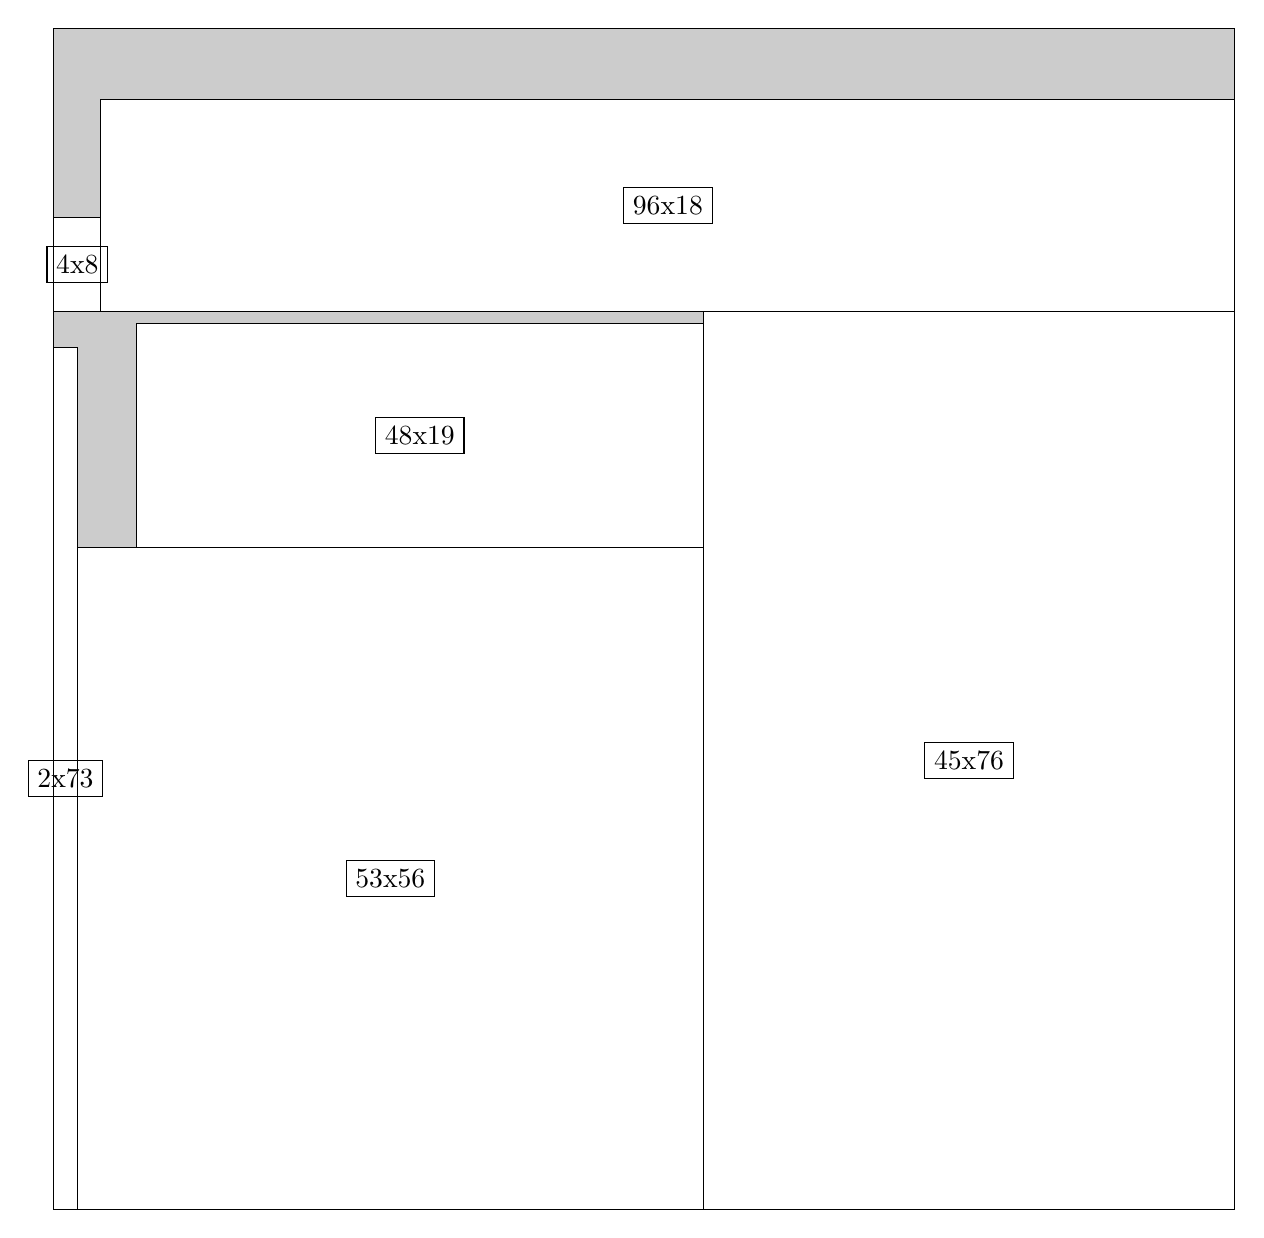
\begin{tikzpicture}[shorten >=1pt,scale=1.0,every node/.style={scale=1.0},->]
\tikzstyle{vertex}=[circle,fill=black!25,minimum size=14pt,inner sep=0pt]
\filldraw[fill=gray!40!white, draw=black] (0,0) rectangle (15.0,15.0);
\foreach \name/\x/\y/\w/\h in {45x76/8.25/0.0/6.75/11.4,53x56/0.3/0.0/7.949999999999999/8.4,48x19/1.05/8.4/7.199999999999999/2.85,2x73/0.0/0.0/0.3/10.95,96x18/0.6/11.4/14.399999999999999/2.6999999999999997,4x8/0.0/11.4/0.6/1.2}
\filldraw[fill=white!40!white, draw=black] (\x,\y) rectangle node[draw] (\name) {\name} ++(\w,\h);
\end{tikzpicture}


w =45 , h =76 , x =55 , y =0 , v =3420
\par
w =53 , h =56 , x =2 , y =0 , v =2968
\par
w =48 , h =19 , x =7 , y =56 , v =912
\par
w =2 , h =73 , x =0 , y =0 , v =146
\par
w =96 , h =18 , x =4 , y =76 , v =1728
\par
w =4 , h =8 , x =0 , y =76 , v =32
\par
\newpage


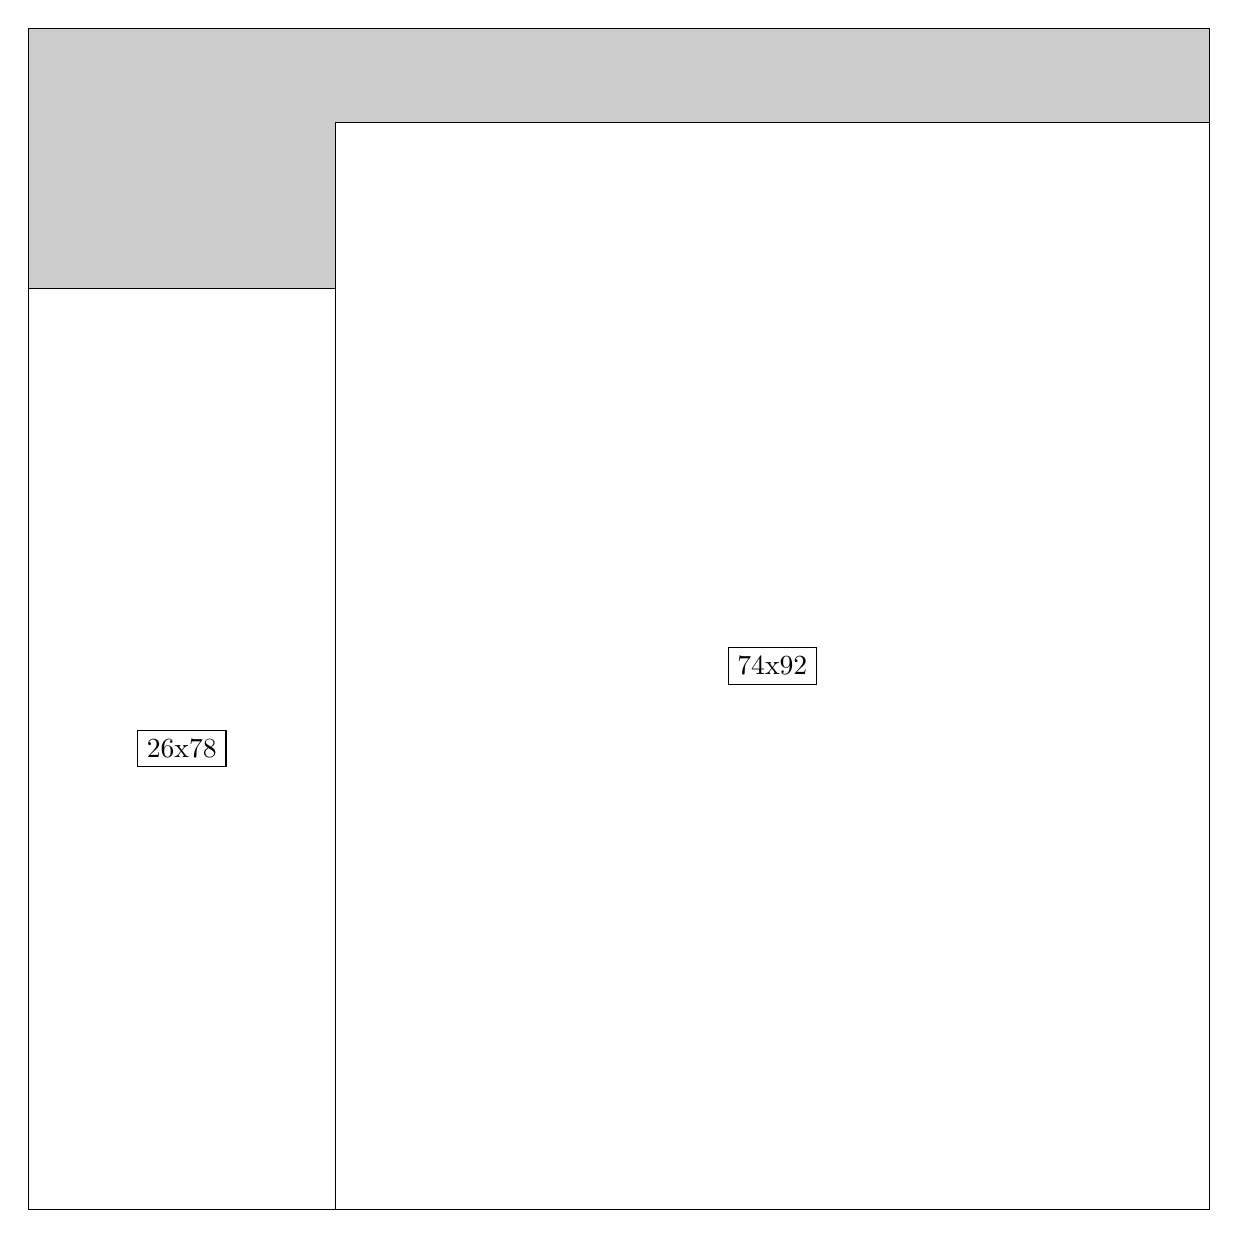
\begin{tikzpicture}[shorten >=1pt,scale=1.0,every node/.style={scale=1.0},->]
\tikzstyle{vertex}=[circle,fill=black!25,minimum size=14pt,inner sep=0pt]
\filldraw[fill=gray!40!white, draw=black] (0,0) rectangle (15.0,15.0);
\foreach \name/\x/\y/\w/\h in {74x92/3.9/0.0/11.1/13.799999999999999,26x78/0.0/0.0/3.9/11.7}
\filldraw[fill=white!40!white, draw=black] (\x,\y) rectangle node[draw] (\name) {\name} ++(\w,\h);
\end{tikzpicture}


w =74 , h =92 , x =26 , y =0 , v =6808
\par
w =26 , h =78 , x =0 , y =0 , v =2028
\par
\newpage


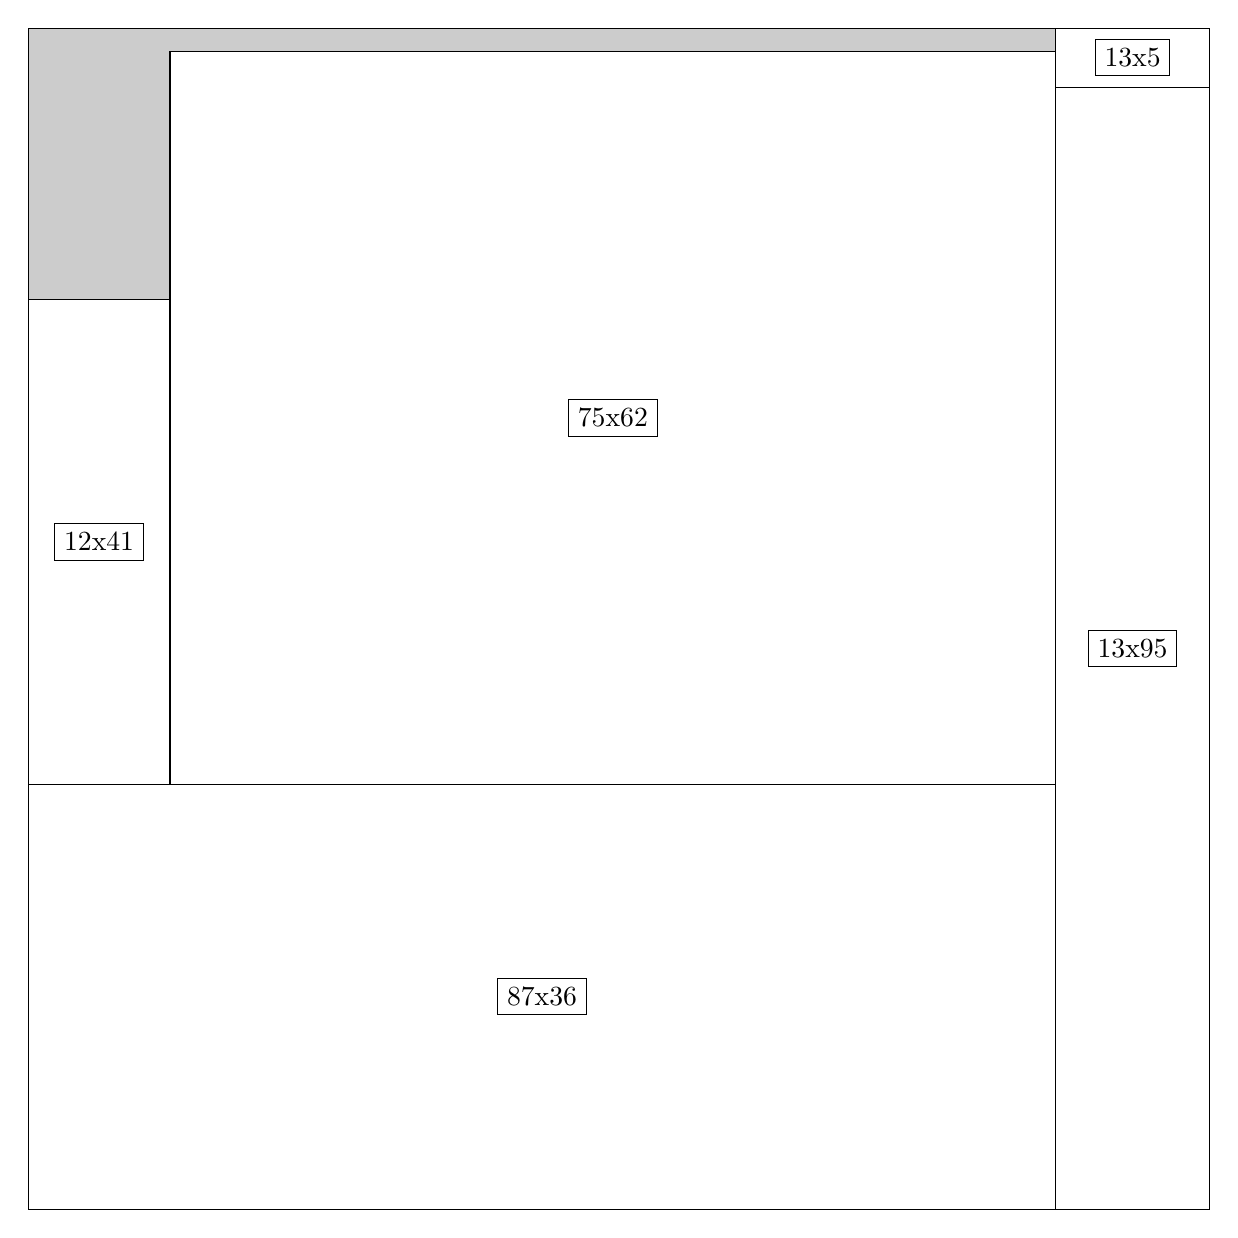
\begin{tikzpicture}[shorten >=1pt,scale=1.0,every node/.style={scale=1.0},->]
\tikzstyle{vertex}=[circle,fill=black!25,minimum size=14pt,inner sep=0pt]
\filldraw[fill=gray!40!white, draw=black] (0,0) rectangle (15.0,15.0);
\foreach \name/\x/\y/\w/\h in {13x95/13.049999999999999/0.0/1.95/14.25,13x5/13.049999999999999/14.25/1.95/0.75,87x36/0.0/0.0/13.049999999999999/5.3999999999999995,75x62/1.7999999999999998/5.3999999999999995/11.25/9.299999999999999,12x41/0.0/5.3999999999999995/1.7999999999999998/6.1499999999999995}
\filldraw[fill=white!40!white, draw=black] (\x,\y) rectangle node[draw] (\name) {\name} ++(\w,\h);
\end{tikzpicture}


w =13 , h =95 , x =87 , y =0 , v =1235
\par
w =13 , h =5 , x =87 , y =95 , v =65
\par
w =87 , h =36 , x =0 , y =0 , v =3132
\par
w =75 , h =62 , x =12 , y =36 , v =4650
\par
w =12 , h =41 , x =0 , y =36 , v =492
\par
\newpage


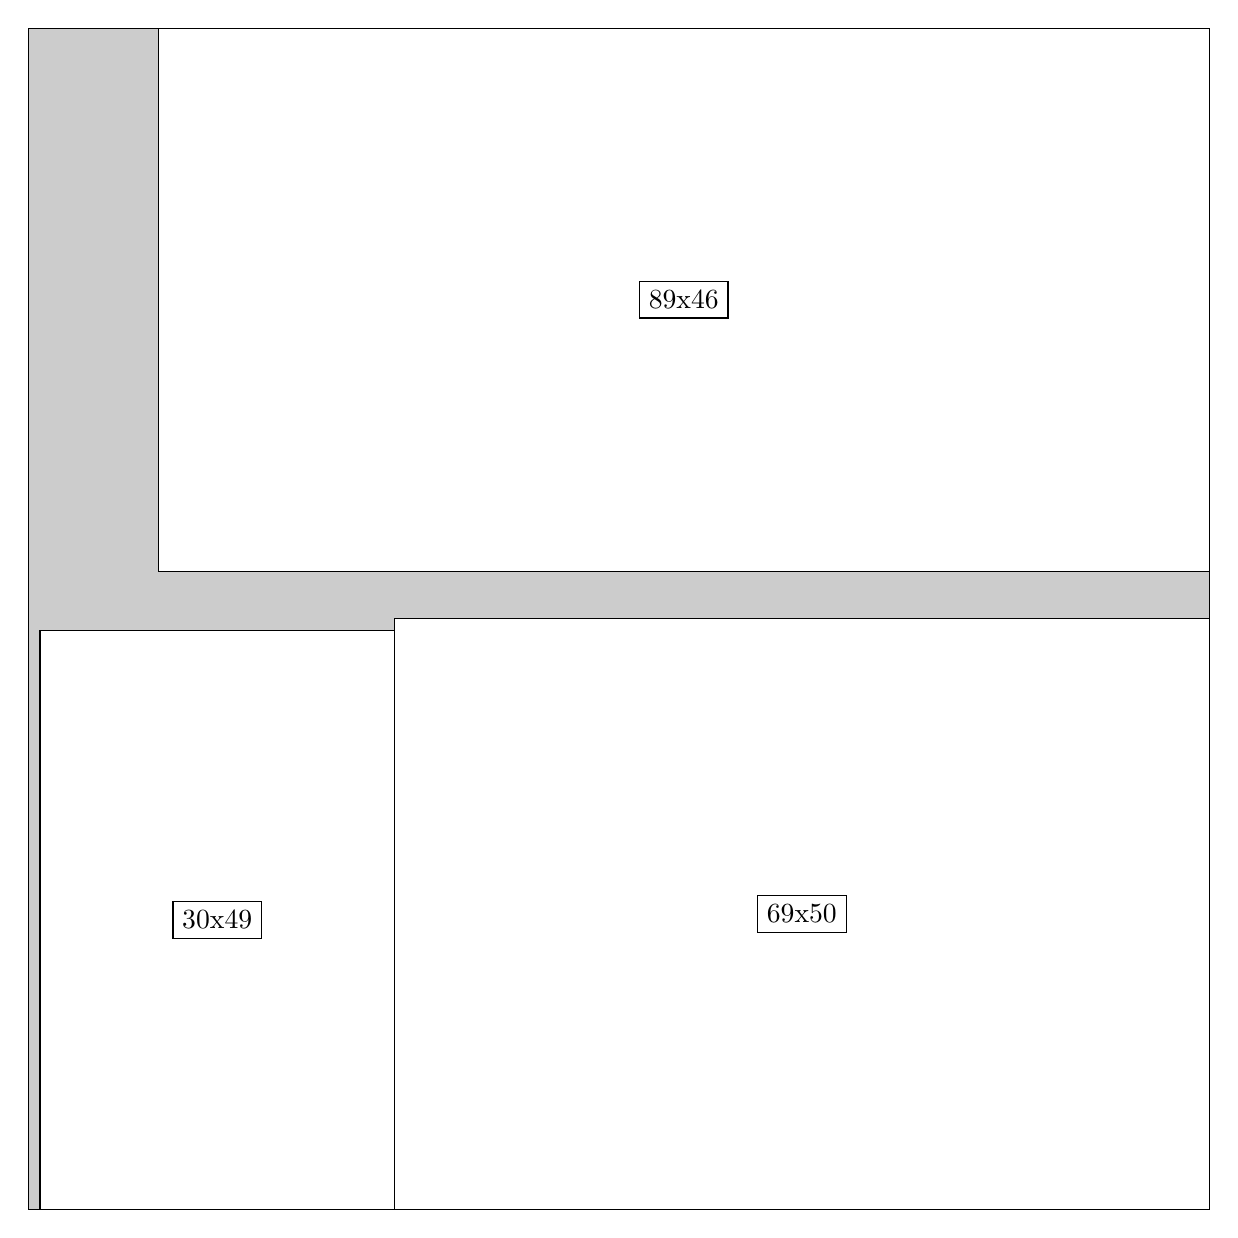
\begin{tikzpicture}[shorten >=1pt,scale=1.0,every node/.style={scale=1.0},->]
\tikzstyle{vertex}=[circle,fill=black!25,minimum size=14pt,inner sep=0pt]
\filldraw[fill=gray!40!white, draw=black] (0,0) rectangle (15.0,15.0);
\foreach \name/\x/\y/\w/\h in {69x50/4.6499999999999995/0.0/10.35/7.5,30x49/0.15/0.0/4.5/7.35,89x46/1.65/8.1/13.35/6.8999999999999995}
\filldraw[fill=white!40!white, draw=black] (\x,\y) rectangle node[draw] (\name) {\name} ++(\w,\h);
\end{tikzpicture}


w =69 , h =50 , x =31 , y =0 , v =3450
\par
w =30 , h =49 , x =1 , y =0 , v =1470
\par
w =89 , h =46 , x =11 , y =54 , v =4094
\par
\newpage


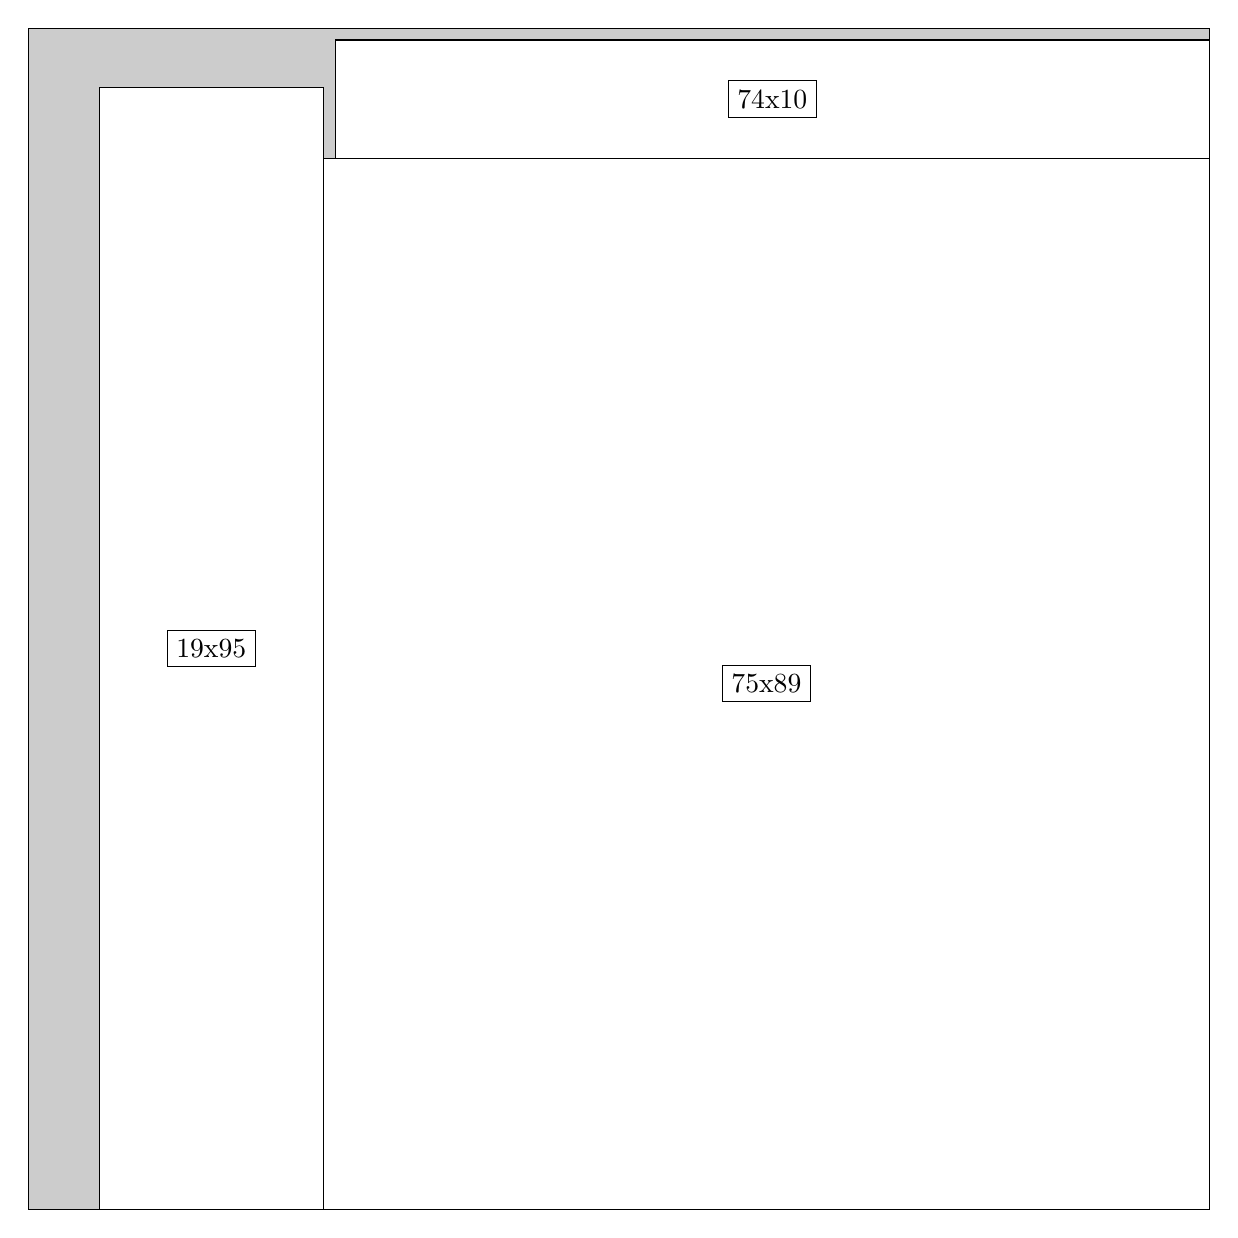
\begin{tikzpicture}[shorten >=1pt,scale=1.0,every node/.style={scale=1.0},->]
\tikzstyle{vertex}=[circle,fill=black!25,minimum size=14pt,inner sep=0pt]
\filldraw[fill=gray!40!white, draw=black] (0,0) rectangle (15.0,15.0);
\foreach \name/\x/\y/\w/\h in {75x89/3.75/0.0/11.25/13.35,74x10/3.9/13.35/11.1/1.5,19x95/0.8999999999999999/0.0/2.85/14.25}
\filldraw[fill=white!40!white, draw=black] (\x,\y) rectangle node[draw] (\name) {\name} ++(\w,\h);
\end{tikzpicture}


w =75 , h =89 , x =25 , y =0 , v =6675
\par
w =74 , h =10 , x =26 , y =89 , v =740
\par
w =19 , h =95 , x =6 , y =0 , v =1805
\par
\newpage


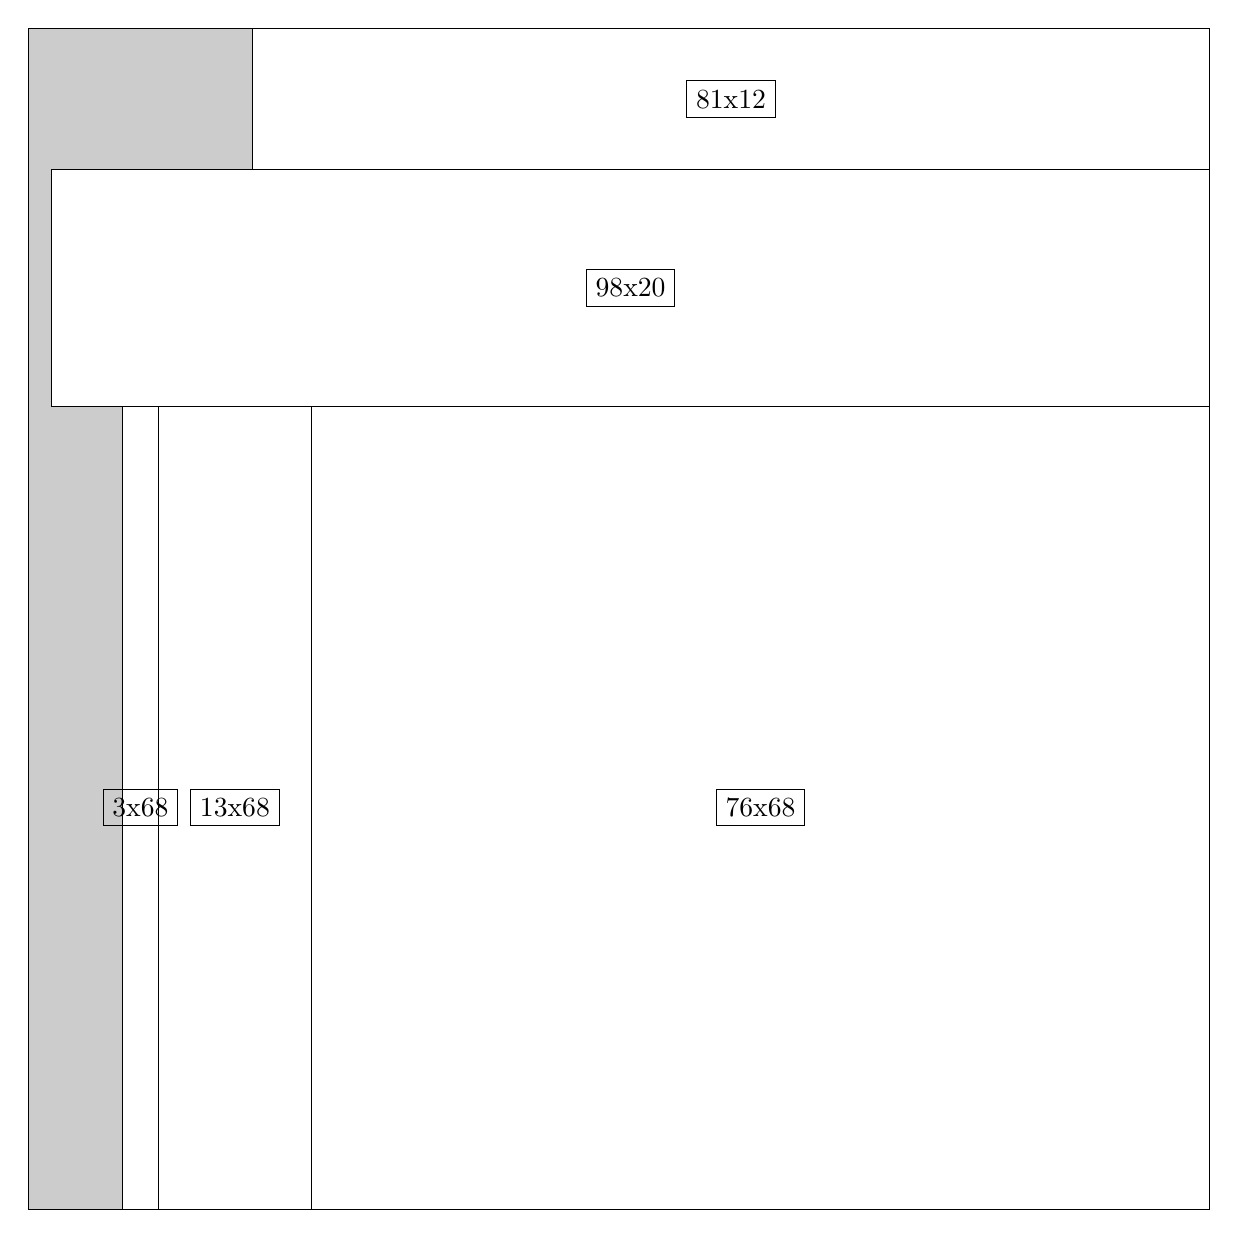
\begin{tikzpicture}[shorten >=1pt,scale=1.0,every node/.style={scale=1.0},->]
\tikzstyle{vertex}=[circle,fill=black!25,minimum size=14pt,inner sep=0pt]
\filldraw[fill=gray!40!white, draw=black] (0,0) rectangle (15.0,15.0);
\foreach \name/\x/\y/\w/\h in {76x68/3.5999999999999996/0.0/11.4/10.2,13x68/1.65/0.0/1.95/10.2,3x68/1.2/0.0/0.44999999999999996/10.2,98x20/0.3/10.2/14.7/3.0,81x12/2.85/13.2/12.15/1.7999999999999998}
\filldraw[fill=white!40!white, draw=black] (\x,\y) rectangle node[draw] (\name) {\name} ++(\w,\h);
\end{tikzpicture}


w =76 , h =68 , x =24 , y =0 , v =5168
\par
w =13 , h =68 , x =11 , y =0 , v =884
\par
w =3 , h =68 , x =8 , y =0 , v =204
\par
w =98 , h =20 , x =2 , y =68 , v =1960
\par
w =81 , h =12 , x =19 , y =88 , v =972
\par
\newpage


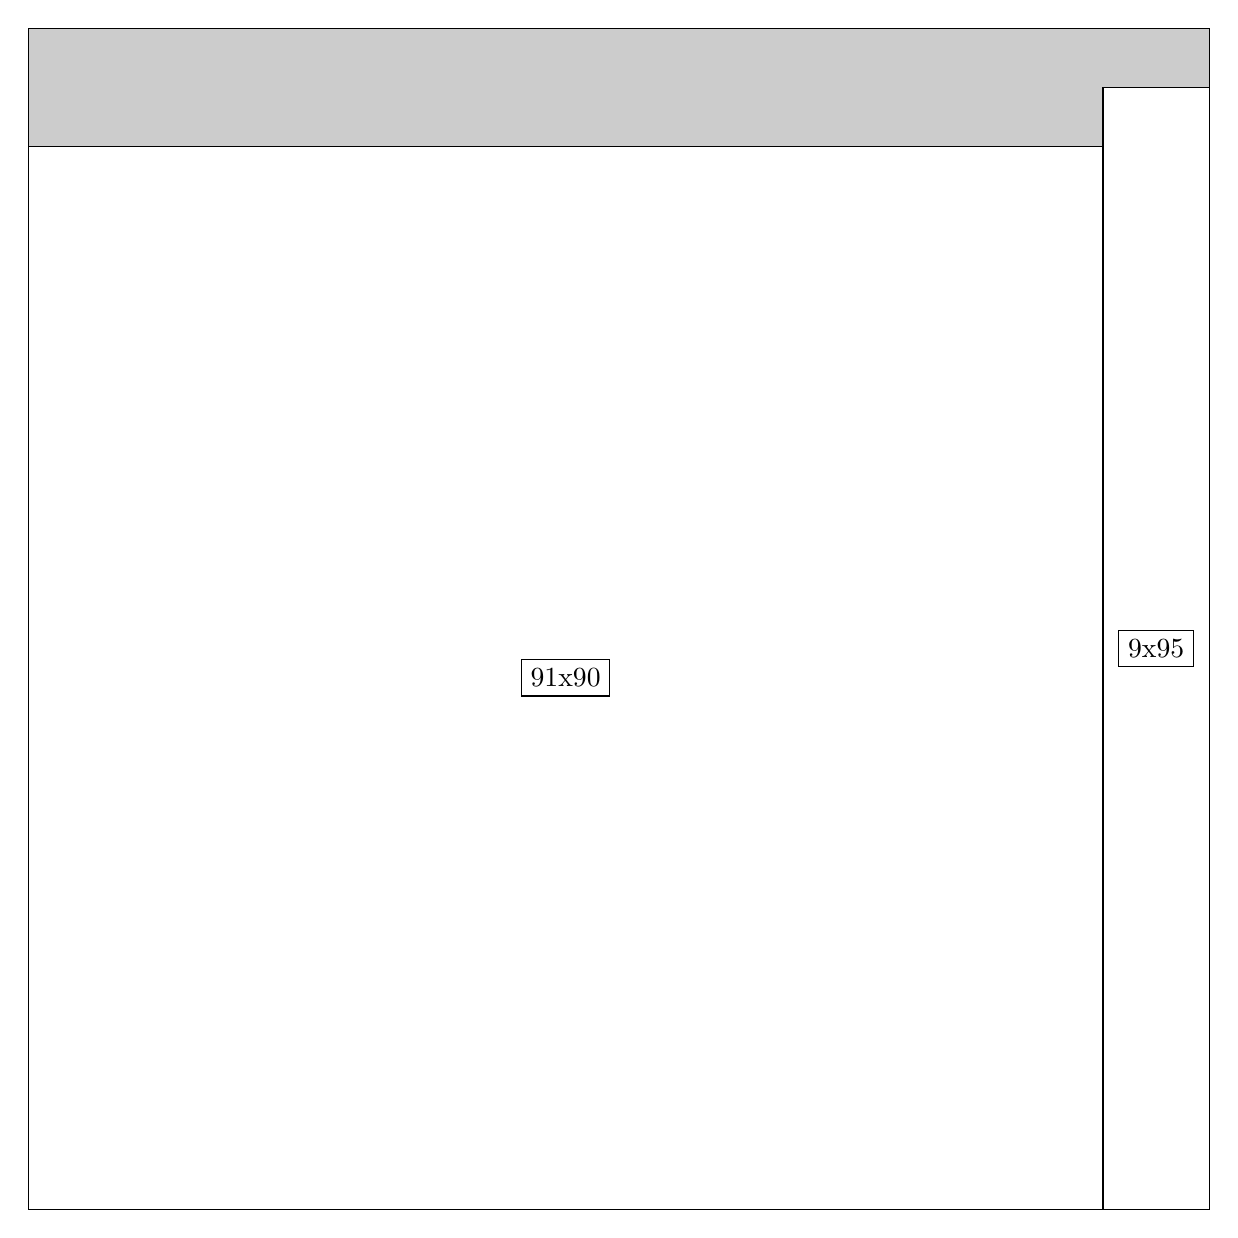
\begin{tikzpicture}[shorten >=1pt,scale=1.0,every node/.style={scale=1.0},->]
\tikzstyle{vertex}=[circle,fill=black!25,minimum size=14pt,inner sep=0pt]
\filldraw[fill=gray!40!white, draw=black] (0,0) rectangle (15.0,15.0);
\foreach \name/\x/\y/\w/\h in {9x95/13.65/0.0/1.3499999999999999/14.25,91x90/0.0/0.0/13.65/13.5}
\filldraw[fill=white!40!white, draw=black] (\x,\y) rectangle node[draw] (\name) {\name} ++(\w,\h);
\end{tikzpicture}


w =9 , h =95 , x =91 , y =0 , v =855
\par
w =91 , h =90 , x =0 , y =0 , v =8190
\par
\newpage


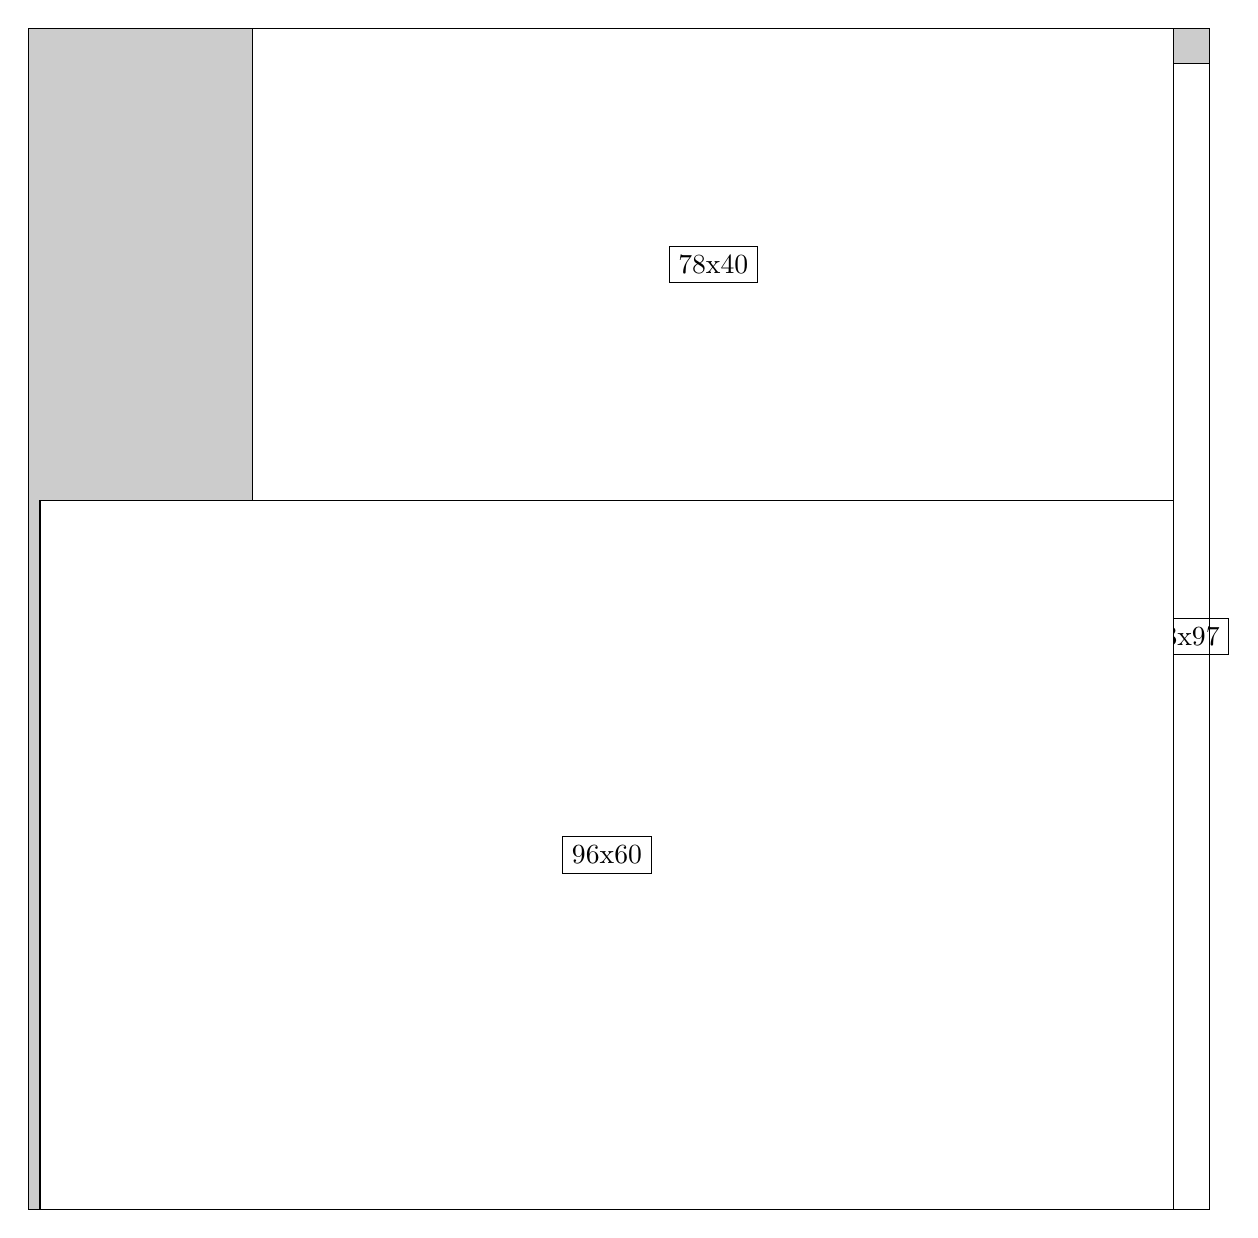
\begin{tikzpicture}[shorten >=1pt,scale=1.0,every node/.style={scale=1.0},->]
\tikzstyle{vertex}=[circle,fill=black!25,minimum size=14pt,inner sep=0pt]
\filldraw[fill=gray!40!white, draw=black] (0,0) rectangle (15.0,15.0);
\foreach \name/\x/\y/\w/\h in {3x97/14.549999999999999/0.0/0.44999999999999996/14.549999999999999,96x60/0.15/0.0/14.399999999999999/9.0,78x40/2.85/9.0/11.7/6.0}
\filldraw[fill=white!40!white, draw=black] (\x,\y) rectangle node[draw] (\name) {\name} ++(\w,\h);
\end{tikzpicture}


w =3 , h =97 , x =97 , y =0 , v =291
\par
w =96 , h =60 , x =1 , y =0 , v =5760
\par
w =78 , h =40 , x =19 , y =60 , v =3120
\par
\newpage


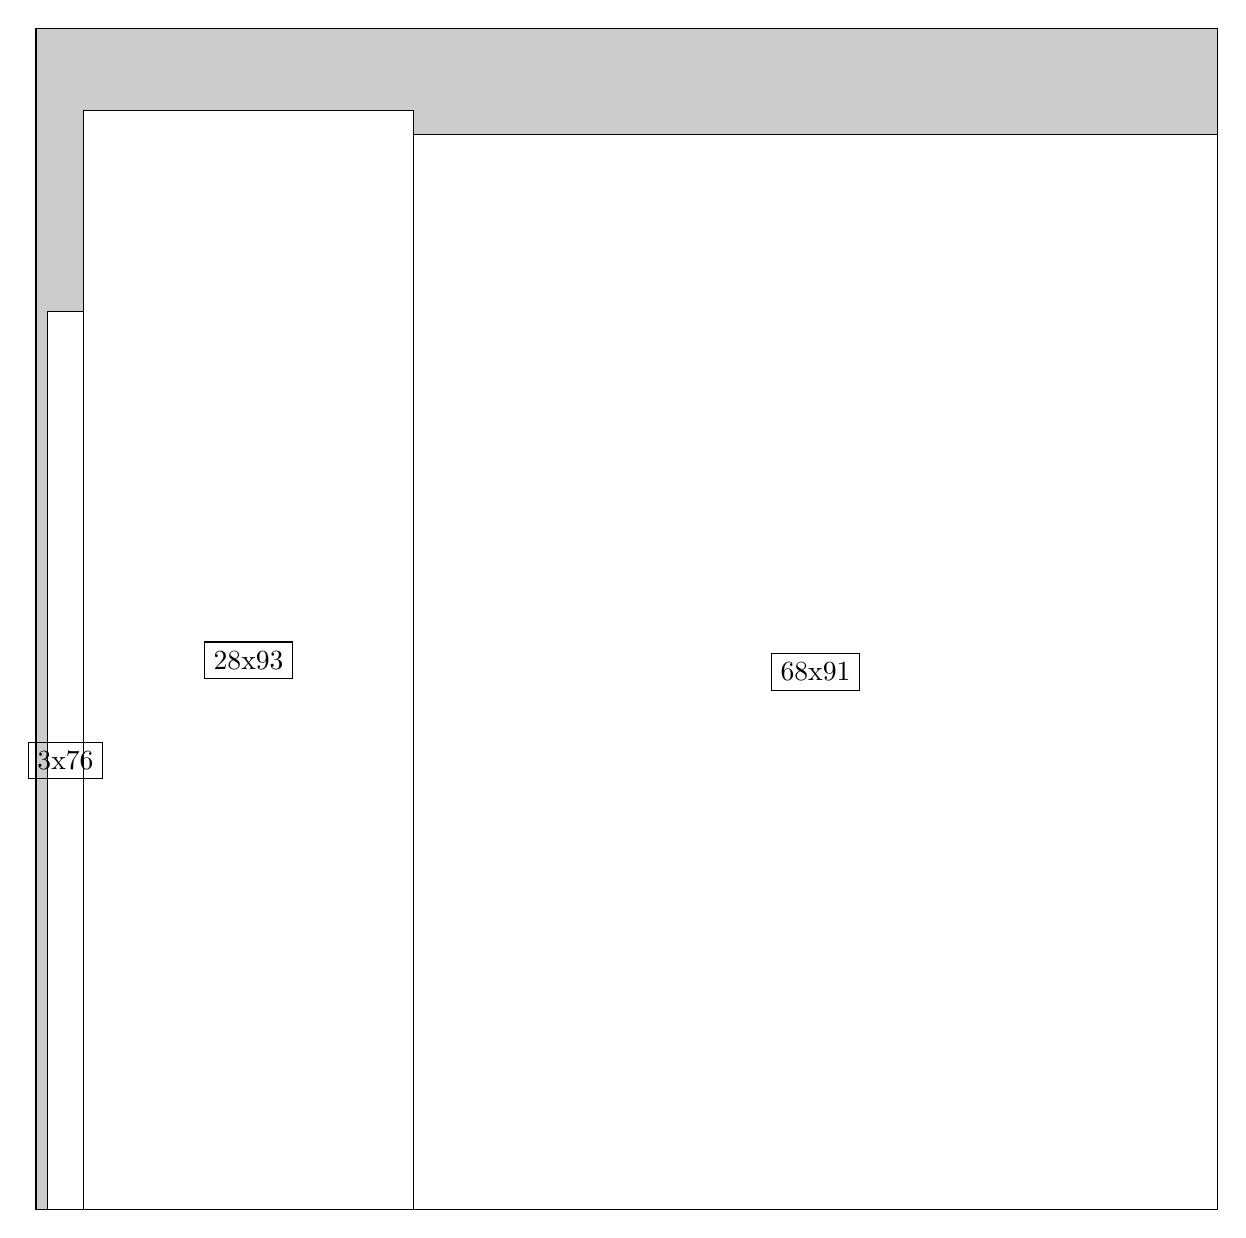
\begin{tikzpicture}[shorten >=1pt,scale=1.0,every node/.style={scale=1.0},->]
\tikzstyle{vertex}=[circle,fill=black!25,minimum size=14pt,inner sep=0pt]
\filldraw[fill=gray!40!white, draw=black] (0,0) rectangle (15.0,15.0);
\foreach \name/\x/\y/\w/\h in {68x91/4.8/0.0/10.2/13.65,28x93/0.6/0.0/4.2/13.95,3x76/0.15/0.0/0.44999999999999996/11.4}
\filldraw[fill=white!40!white, draw=black] (\x,\y) rectangle node[draw] (\name) {\name} ++(\w,\h);
\end{tikzpicture}


w =68 , h =91 , x =32 , y =0 , v =6188
\par
w =28 , h =93 , x =4 , y =0 , v =2604
\par
w =3 , h =76 , x =1 , y =0 , v =228
\par
\newpage


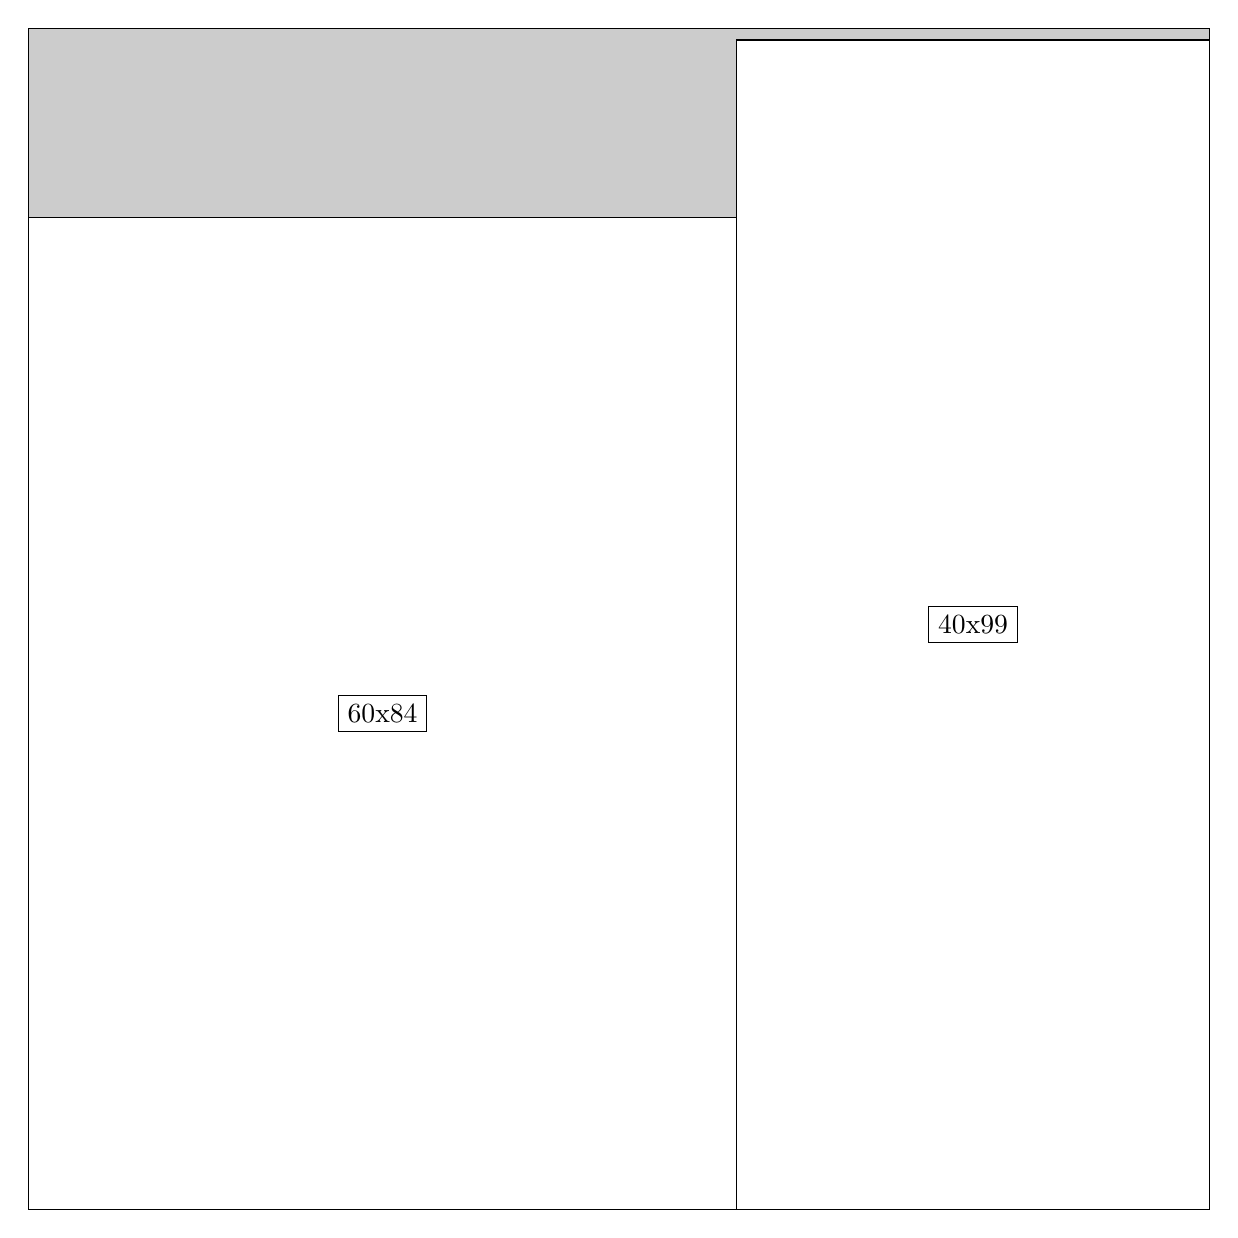
\begin{tikzpicture}[shorten >=1pt,scale=1.0,every node/.style={scale=1.0},->]
\tikzstyle{vertex}=[circle,fill=black!25,minimum size=14pt,inner sep=0pt]
\filldraw[fill=gray!40!white, draw=black] (0,0) rectangle (15.0,15.0);
\foreach \name/\x/\y/\w/\h in {40x99/9.0/0.0/6.0/14.85,60x84/0.0/0.0/9.0/12.6}
\filldraw[fill=white!40!white, draw=black] (\x,\y) rectangle node[draw] (\name) {\name} ++(\w,\h);
\end{tikzpicture}


w =40 , h =99 , x =60 , y =0 , v =3960
\par
w =60 , h =84 , x =0 , y =0 , v =5040
\par
\newpage


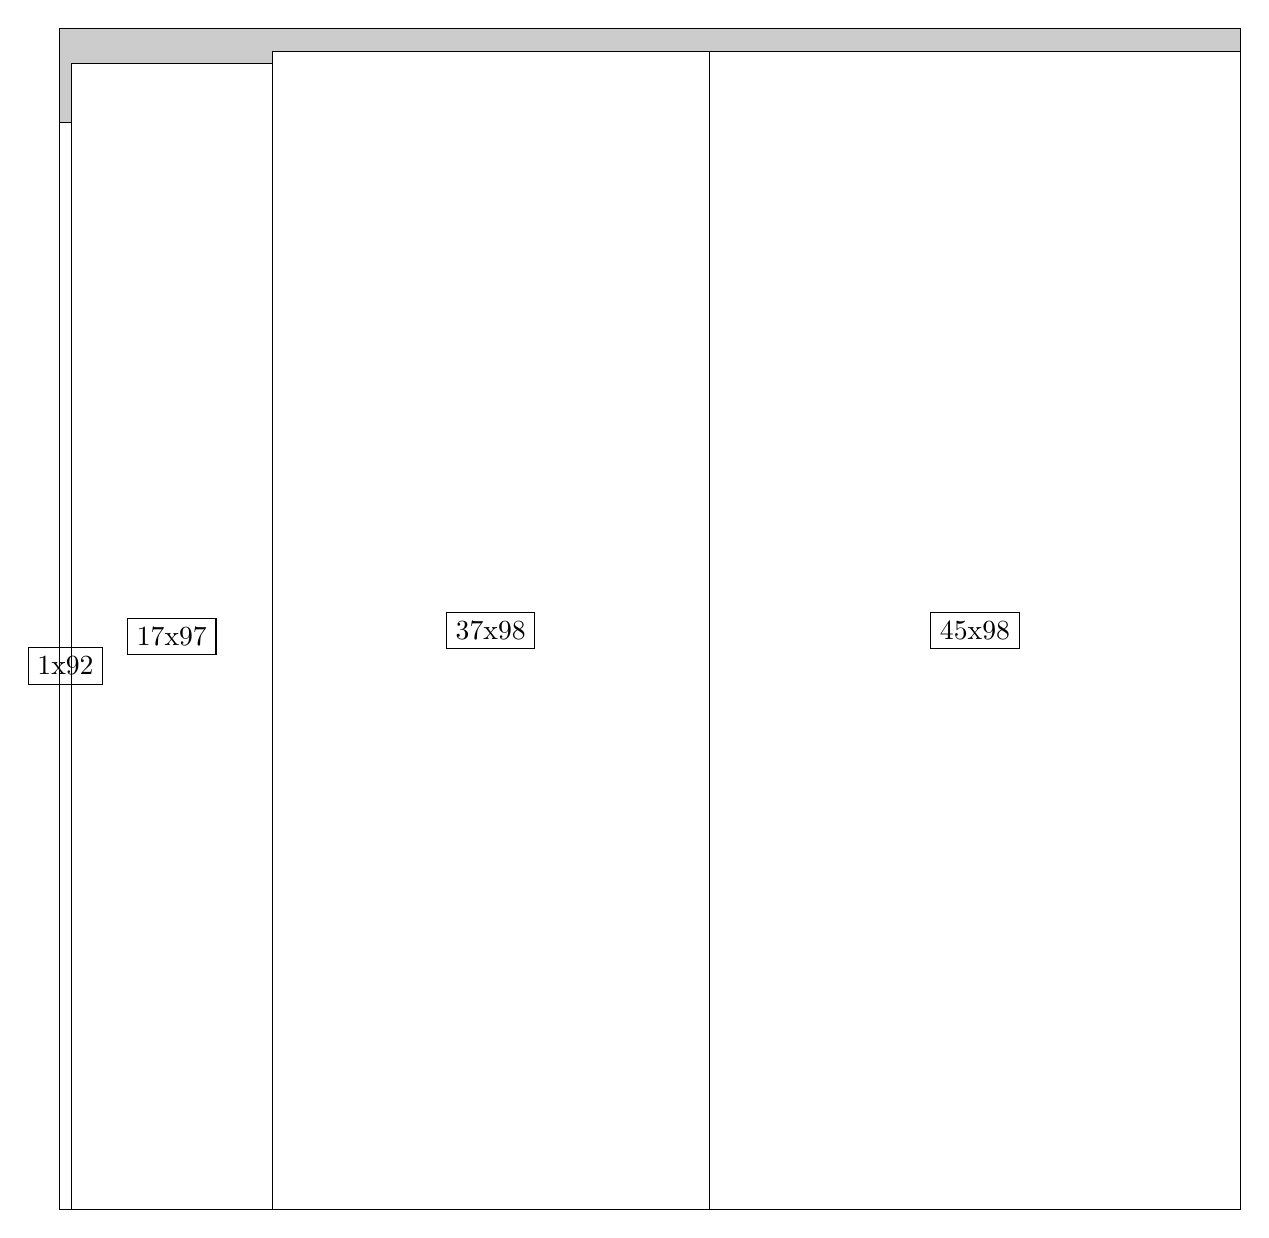
\begin{tikzpicture}[shorten >=1pt,scale=1.0,every node/.style={scale=1.0},->]
\tikzstyle{vertex}=[circle,fill=black!25,minimum size=14pt,inner sep=0pt]
\filldraw[fill=gray!40!white, draw=black] (0,0) rectangle (15.0,15.0);
\foreach \name/\x/\y/\w/\h in {45x98/8.25/0.0/6.75/14.7,37x98/2.6999999999999997/0.0/5.55/14.7,17x97/0.15/0.0/2.55/14.549999999999999,1x92/0.0/0.0/0.15/13.799999999999999}
\filldraw[fill=white!40!white, draw=black] (\x,\y) rectangle node[draw] (\name) {\name} ++(\w,\h);
\end{tikzpicture}


w =45 , h =98 , x =55 , y =0 , v =4410
\par
w =37 , h =98 , x =18 , y =0 , v =3626
\par
w =17 , h =97 , x =1 , y =0 , v =1649
\par
w =1 , h =92 , x =0 , y =0 , v =92
\par
\newpage


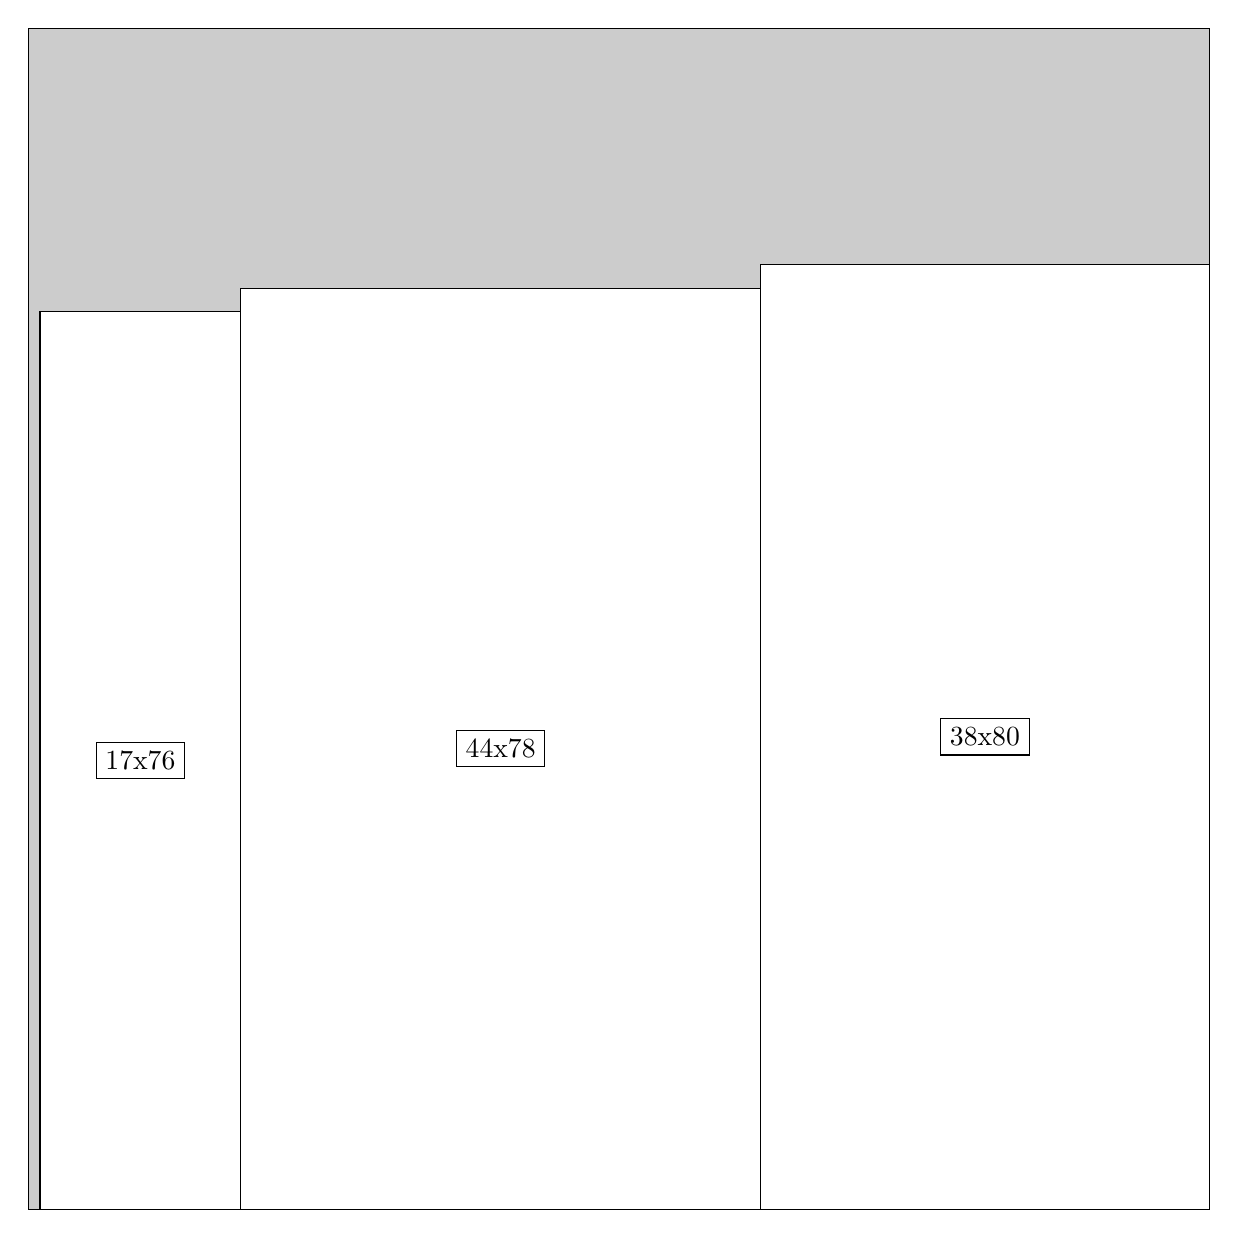
\begin{tikzpicture}[shorten >=1pt,scale=1.0,every node/.style={scale=1.0},->]
\tikzstyle{vertex}=[circle,fill=black!25,minimum size=14pt,inner sep=0pt]
\filldraw[fill=gray!40!white, draw=black] (0,0) rectangle (15.0,15.0);
\foreach \name/\x/\y/\w/\h in {38x80/9.299999999999999/0.0/5.7/12.0,44x78/2.6999999999999997/0.0/6.6/11.7,17x76/0.15/0.0/2.55/11.4}
\filldraw[fill=white!40!white, draw=black] (\x,\y) rectangle node[draw] (\name) {\name} ++(\w,\h);
\end{tikzpicture}


w =38 , h =80 , x =62 , y =0 , v =3040
\par
w =44 , h =78 , x =18 , y =0 , v =3432
\par
w =17 , h =76 , x =1 , y =0 , v =1292
\par
\newpage


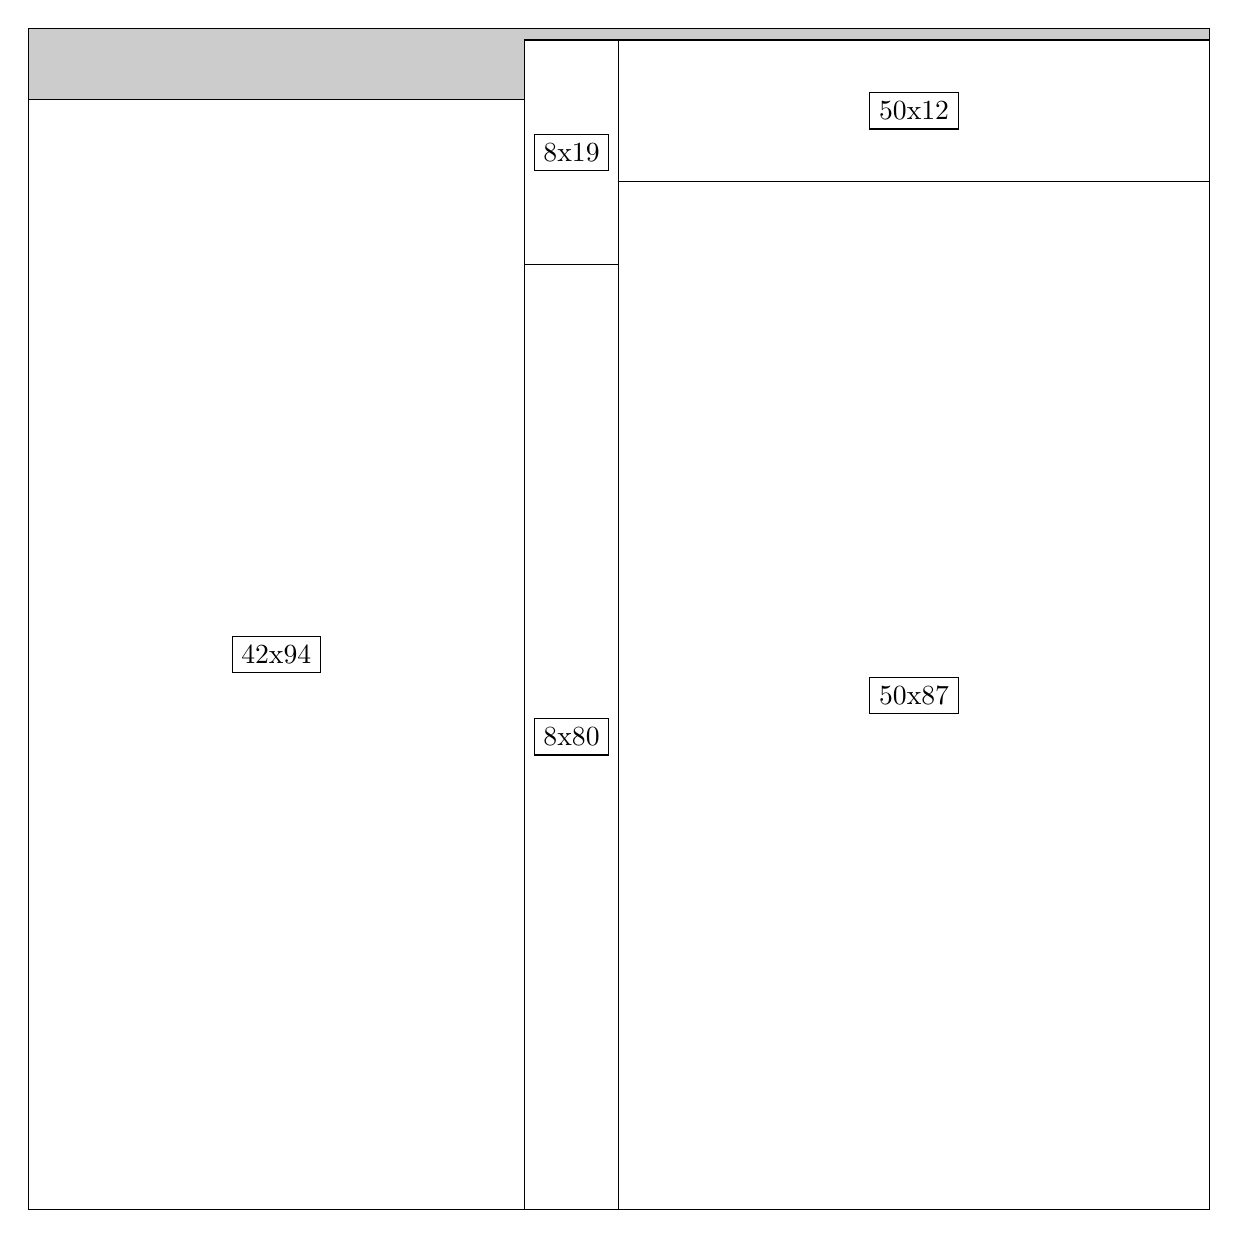
\begin{tikzpicture}[shorten >=1pt,scale=1.0,every node/.style={scale=1.0},->]
\tikzstyle{vertex}=[circle,fill=black!25,minimum size=14pt,inner sep=0pt]
\filldraw[fill=gray!40!white, draw=black] (0,0) rectangle (15.0,15.0);
\foreach \name/\x/\y/\w/\h in {50x87/7.5/0.0/7.5/13.049999999999999,50x12/7.5/13.049999999999999/7.5/1.7999999999999998,8x80/6.3/0.0/1.2/12.0,8x19/6.3/12.0/1.2/2.85,42x94/0.0/0.0/6.3/14.1}
\filldraw[fill=white!40!white, draw=black] (\x,\y) rectangle node[draw] (\name) {\name} ++(\w,\h);
\end{tikzpicture}


w =50 , h =87 , x =50 , y =0 , v =4350
\par
w =50 , h =12 , x =50 , y =87 , v =600
\par
w =8 , h =80 , x =42 , y =0 , v =640
\par
w =8 , h =19 , x =42 , y =80 , v =152
\par
w =42 , h =94 , x =0 , y =0 , v =3948
\par
\newpage


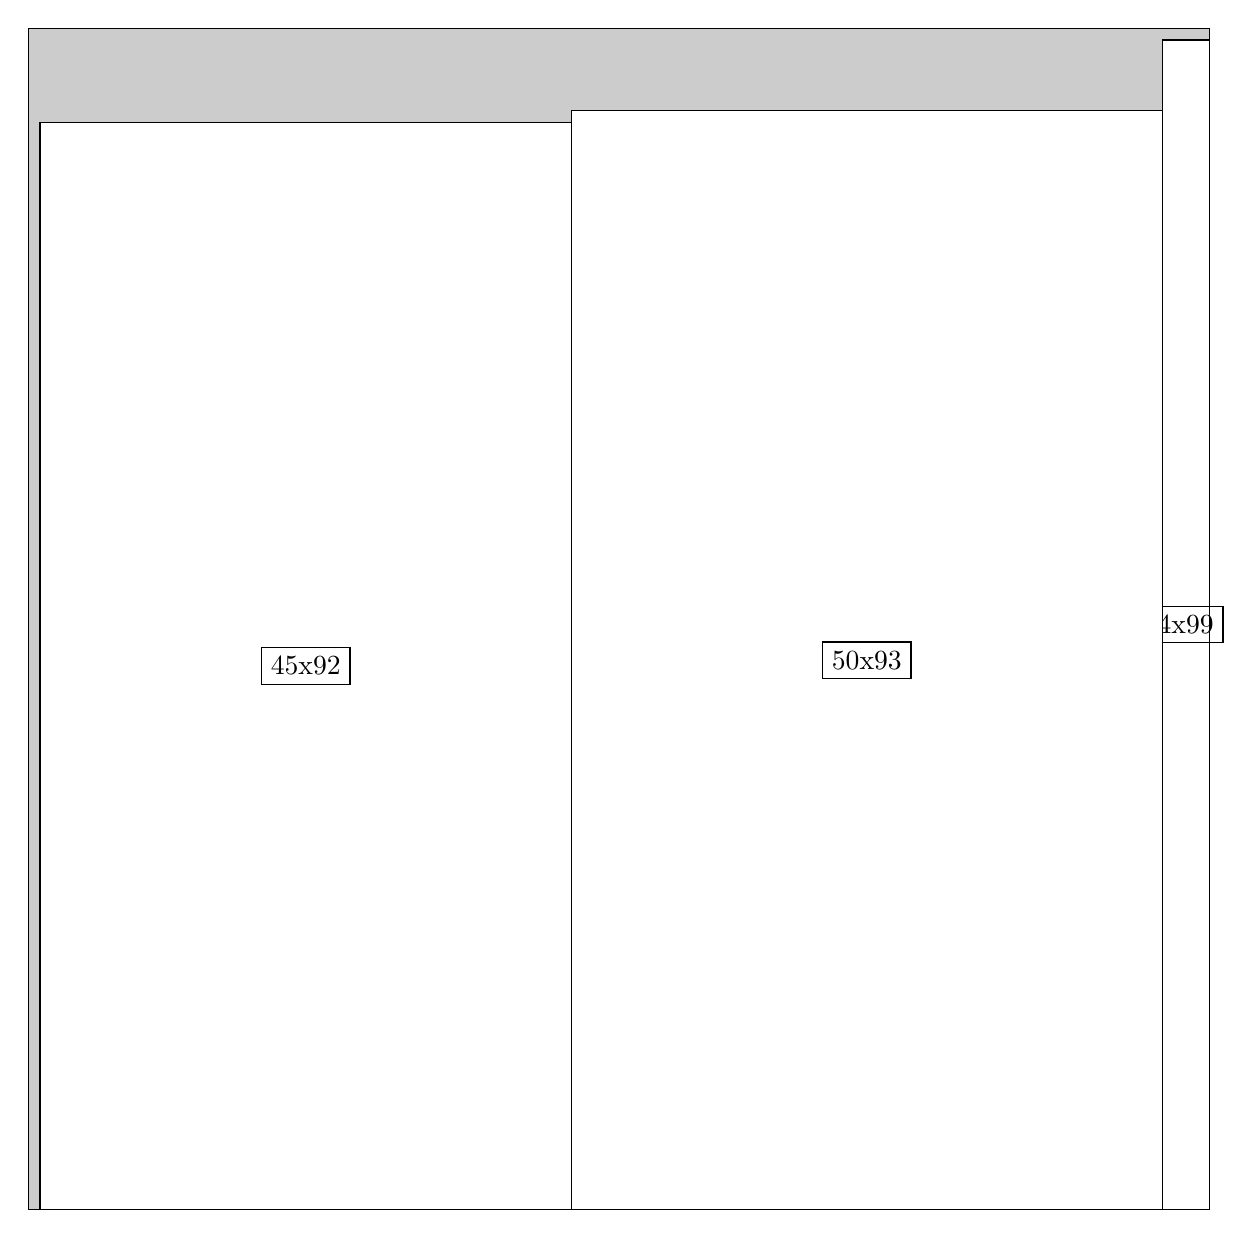
\begin{tikzpicture}[shorten >=1pt,scale=1.0,every node/.style={scale=1.0},->]
\tikzstyle{vertex}=[circle,fill=black!25,minimum size=14pt,inner sep=0pt]
\filldraw[fill=gray!40!white, draw=black] (0,0) rectangle (15.0,15.0);
\foreach \name/\x/\y/\w/\h in {4x99/14.399999999999999/0.0/0.6/14.85,50x93/6.8999999999999995/0.0/7.5/13.95,45x92/0.15/0.0/6.75/13.799999999999999}
\filldraw[fill=white!40!white, draw=black] (\x,\y) rectangle node[draw] (\name) {\name} ++(\w,\h);
\end{tikzpicture}


w =4 , h =99 , x =96 , y =0 , v =396
\par
w =50 , h =93 , x =46 , y =0 , v =4650
\par
w =45 , h =92 , x =1 , y =0 , v =4140
\par
\newpage


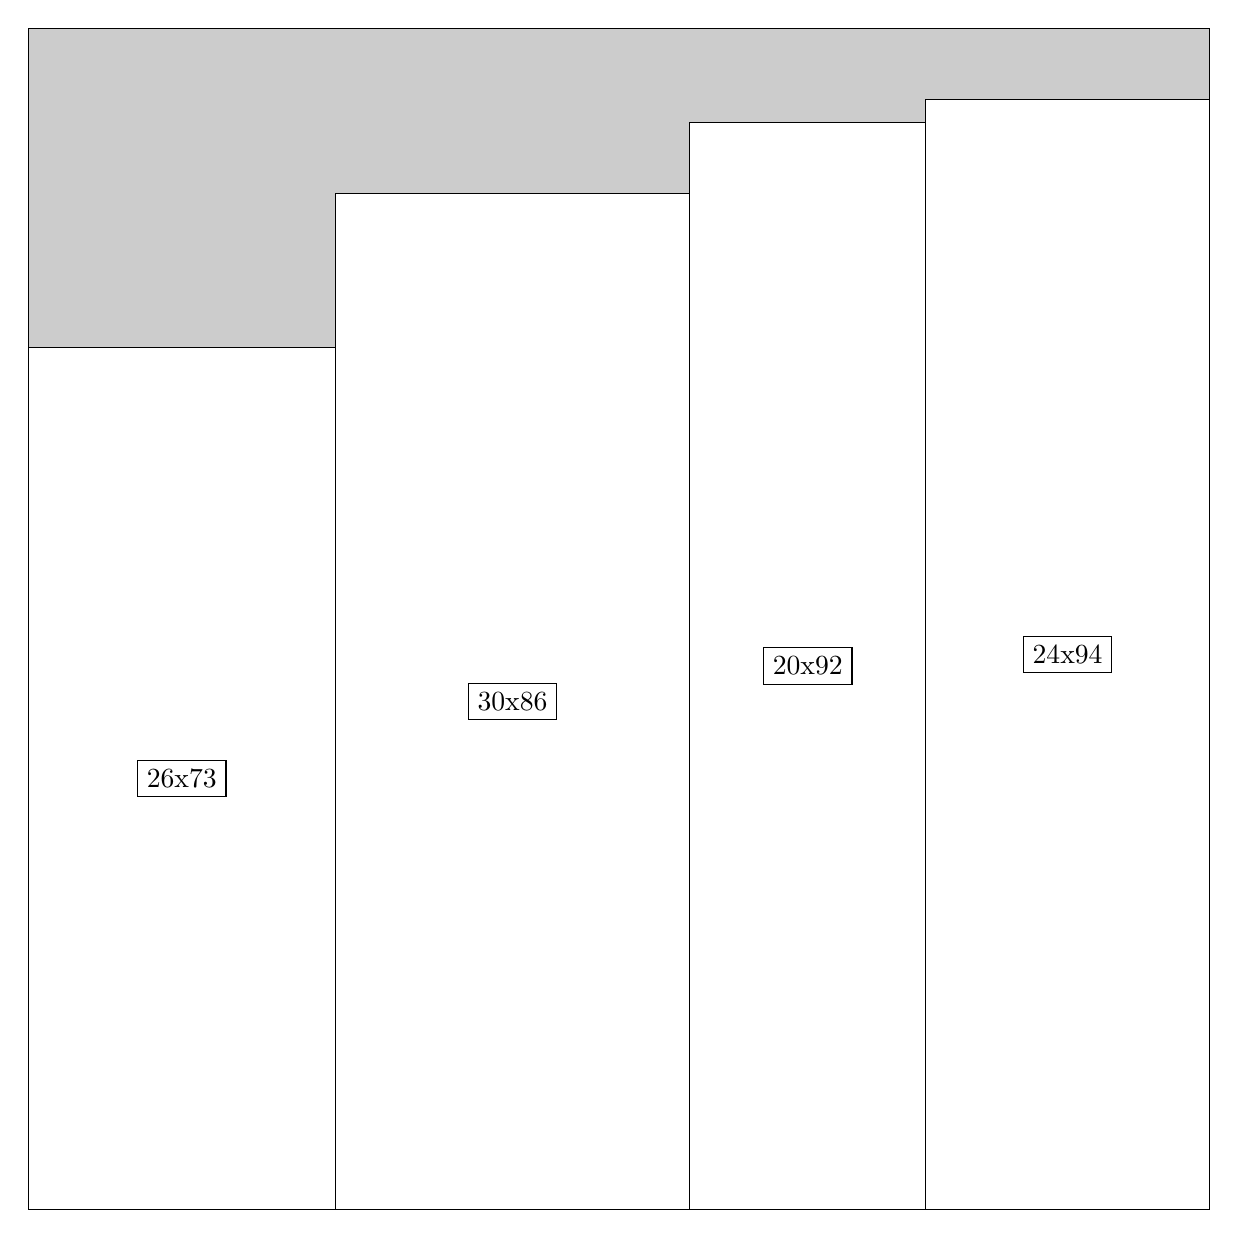
\begin{tikzpicture}[shorten >=1pt,scale=1.0,every node/.style={scale=1.0},->]
\tikzstyle{vertex}=[circle,fill=black!25,minimum size=14pt,inner sep=0pt]
\filldraw[fill=gray!40!white, draw=black] (0,0) rectangle (15.0,15.0);
\foreach \name/\x/\y/\w/\h in {24x94/11.4/0.0/3.5999999999999996/14.1,20x92/8.4/0.0/3.0/13.799999999999999,30x86/3.9/0.0/4.5/12.9,26x73/0.0/0.0/3.9/10.95}
\filldraw[fill=white!40!white, draw=black] (\x,\y) rectangle node[draw] (\name) {\name} ++(\w,\h);
\end{tikzpicture}


w =24 , h =94 , x =76 , y =0 , v =2256
\par
w =20 , h =92 , x =56 , y =0 , v =1840
\par
w =30 , h =86 , x =26 , y =0 , v =2580
\par
w =26 , h =73 , x =0 , y =0 , v =1898
\par
\newpage


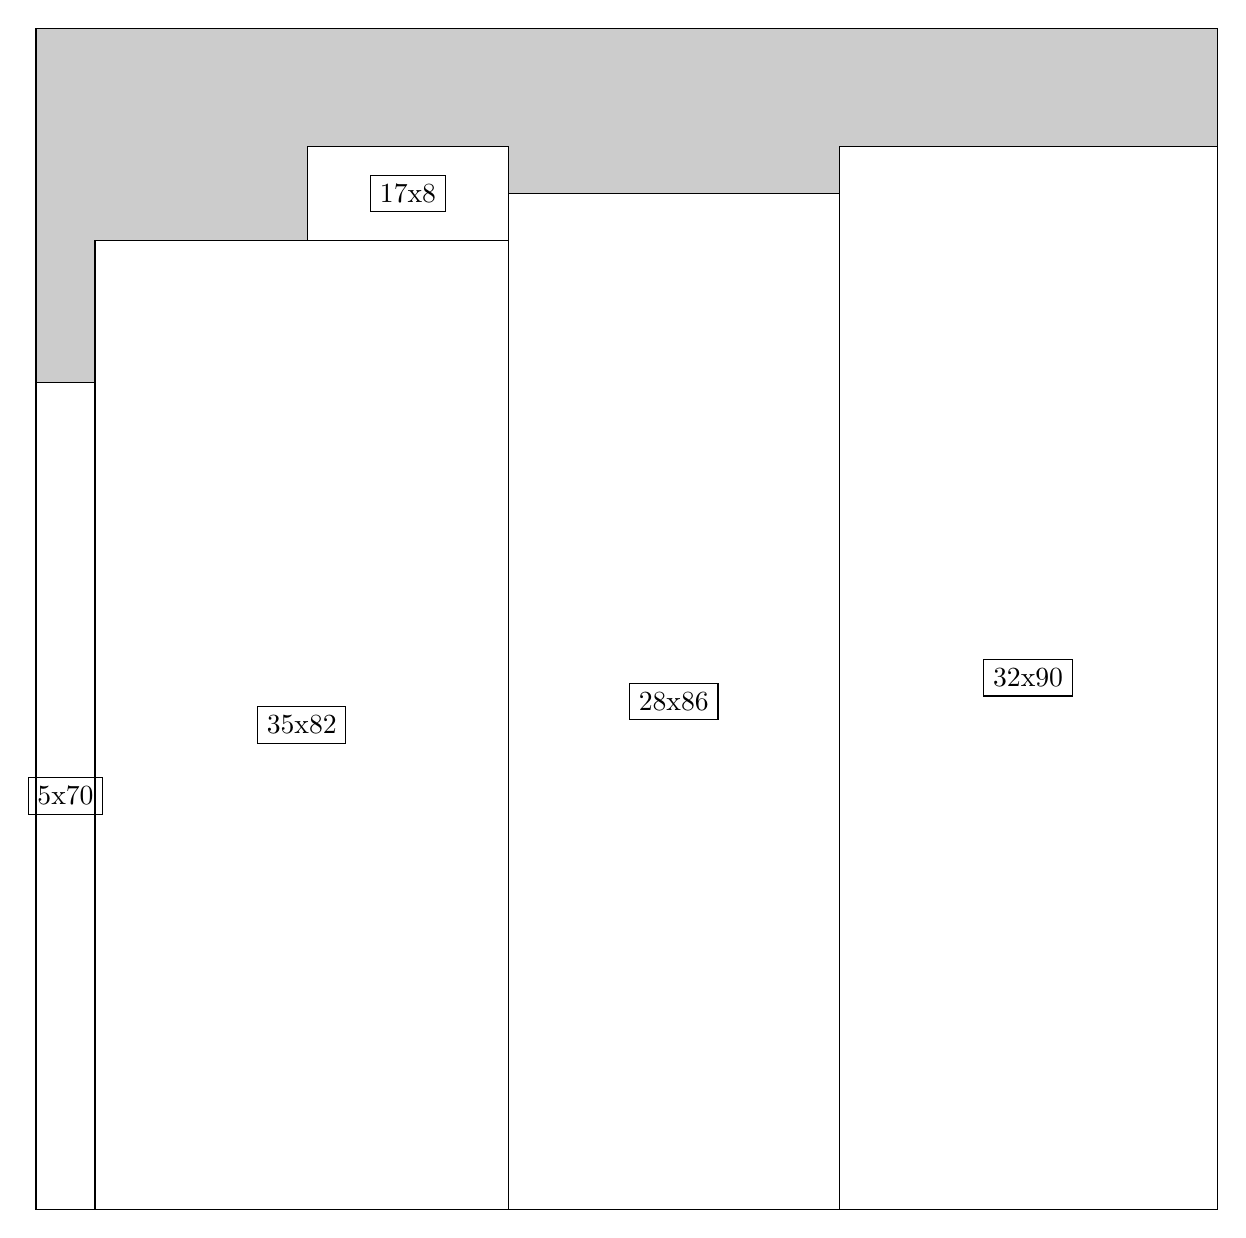
\begin{tikzpicture}[shorten >=1pt,scale=1.0,every node/.style={scale=1.0},->]
\tikzstyle{vertex}=[circle,fill=black!25,minimum size=14pt,inner sep=0pt]
\filldraw[fill=gray!40!white, draw=black] (0,0) rectangle (15.0,15.0);
\foreach \name/\x/\y/\w/\h in {32x90/10.2/0.0/4.8/13.5,28x86/6.0/0.0/4.2/12.9,35x82/0.75/0.0/5.25/12.299999999999999,17x8/3.4499999999999997/12.299999999999999/2.55/1.2,5x70/0.0/0.0/0.75/10.5}
\filldraw[fill=white!40!white, draw=black] (\x,\y) rectangle node[draw] (\name) {\name} ++(\w,\h);
\end{tikzpicture}


w =32 , h =90 , x =68 , y =0 , v =2880
\par
w =28 , h =86 , x =40 , y =0 , v =2408
\par
w =35 , h =82 , x =5 , y =0 , v =2870
\par
w =17 , h =8 , x =23 , y =82 , v =136
\par
w =5 , h =70 , x =0 , y =0 , v =350
\par
\newpage


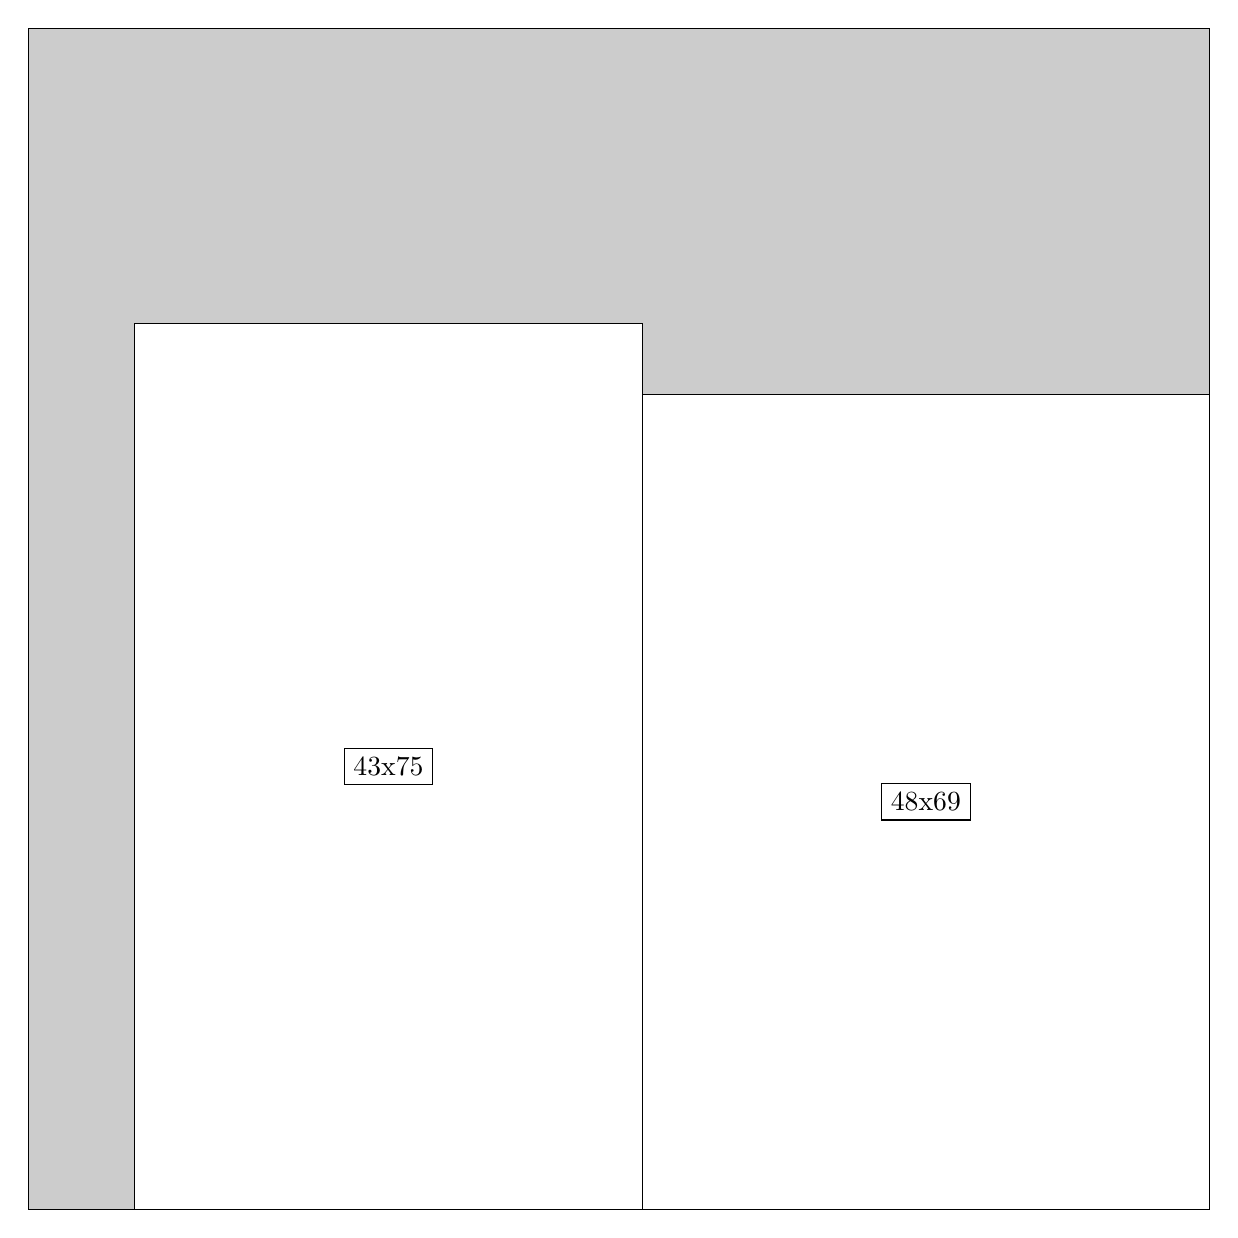
\begin{tikzpicture}[shorten >=1pt,scale=1.0,every node/.style={scale=1.0},->]
\tikzstyle{vertex}=[circle,fill=black!25,minimum size=14pt,inner sep=0pt]
\filldraw[fill=gray!40!white, draw=black] (0,0) rectangle (15.0,15.0);
\foreach \name/\x/\y/\w/\h in {48x69/7.8/0.0/7.199999999999999/10.35,43x75/1.3499999999999999/0.0/6.45/11.25}
\filldraw[fill=white!40!white, draw=black] (\x,\y) rectangle node[draw] (\name) {\name} ++(\w,\h);
\end{tikzpicture}


w =48 , h =69 , x =52 , y =0 , v =3312
\par
w =43 , h =75 , x =9 , y =0 , v =3225
\par
\newpage


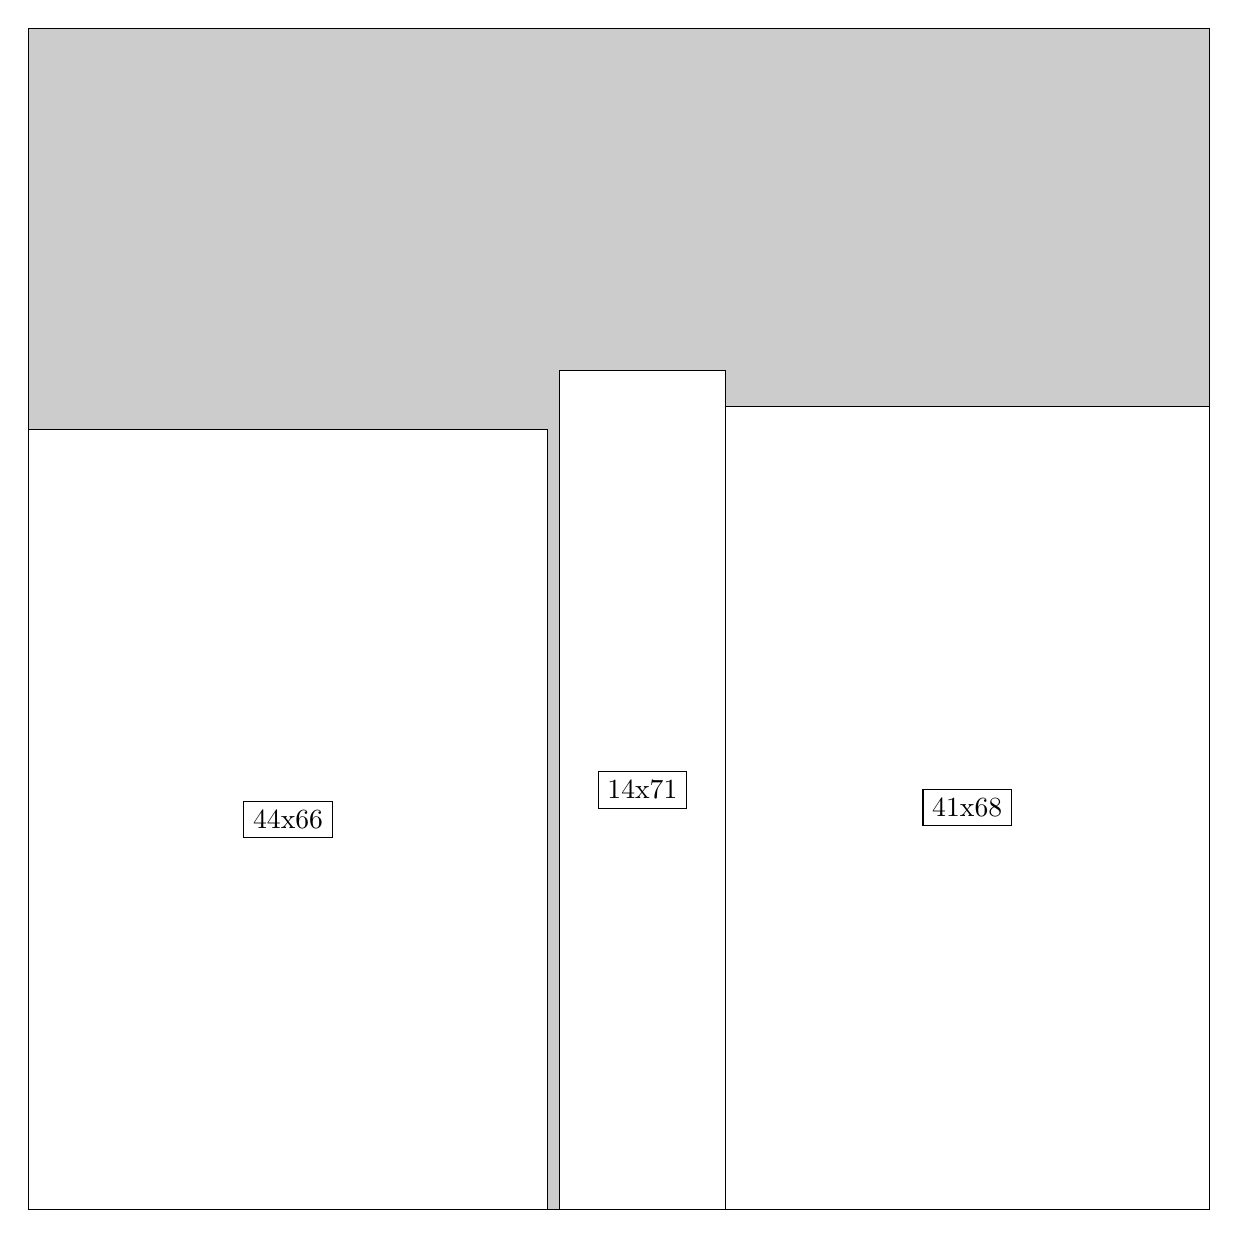
\begin{tikzpicture}[shorten >=1pt,scale=1.0,every node/.style={scale=1.0},->]
\tikzstyle{vertex}=[circle,fill=black!25,minimum size=14pt,inner sep=0pt]
\filldraw[fill=gray!40!white, draw=black] (0,0) rectangle (15.0,15.0);
\foreach \name/\x/\y/\w/\h in {41x68/8.85/0.0/6.1499999999999995/10.2,14x71/6.75/0.0/2.1/10.65,44x66/0.0/0.0/6.6/9.9}
\filldraw[fill=white!40!white, draw=black] (\x,\y) rectangle node[draw] (\name) {\name} ++(\w,\h);
\end{tikzpicture}


w =41 , h =68 , x =59 , y =0 , v =2788
\par
w =14 , h =71 , x =45 , y =0 , v =994
\par
w =44 , h =66 , x =0 , y =0 , v =2904
\par
\newpage


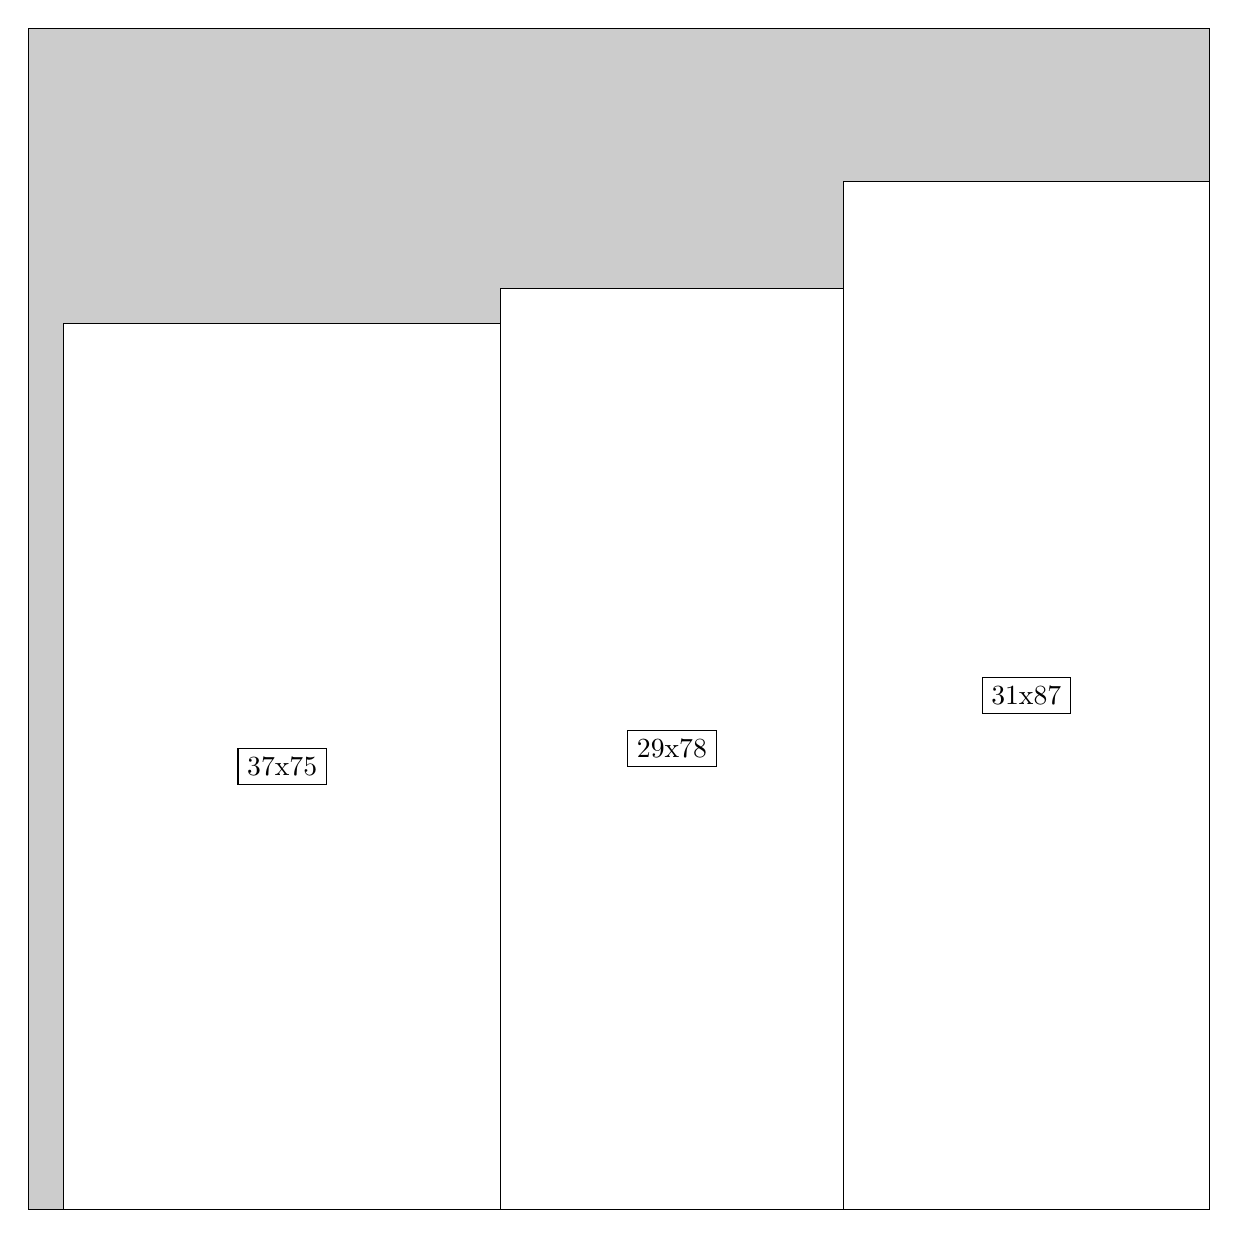
\begin{tikzpicture}[shorten >=1pt,scale=1.0,every node/.style={scale=1.0},->]
\tikzstyle{vertex}=[circle,fill=black!25,minimum size=14pt,inner sep=0pt]
\filldraw[fill=gray!40!white, draw=black] (0,0) rectangle (15.0,15.0);
\foreach \name/\x/\y/\w/\h in {31x87/10.35/0.0/4.6499999999999995/13.049999999999999,29x78/6.0/0.0/4.35/11.7,37x75/0.44999999999999996/0.0/5.55/11.25}
\filldraw[fill=white!40!white, draw=black] (\x,\y) rectangle node[draw] (\name) {\name} ++(\w,\h);
\end{tikzpicture}


w =31 , h =87 , x =69 , y =0 , v =2697
\par
w =29 , h =78 , x =40 , y =0 , v =2262
\par
w =37 , h =75 , x =3 , y =0 , v =2775
\par
\newpage


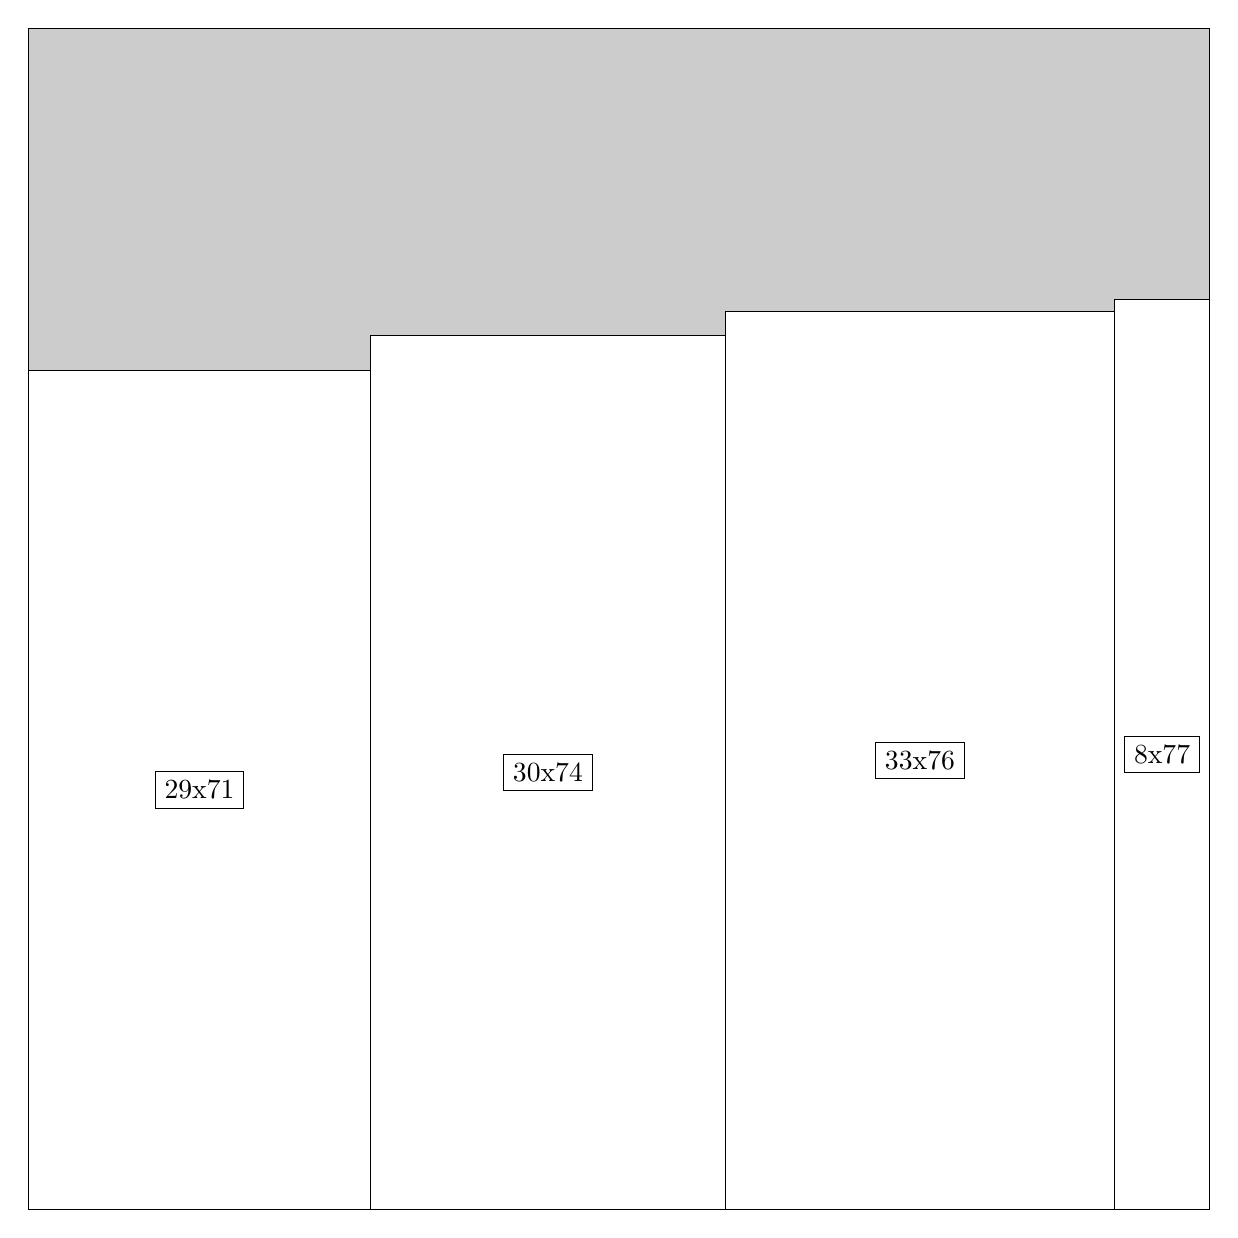
\begin{tikzpicture}[shorten >=1pt,scale=1.0,every node/.style={scale=1.0},->]
\tikzstyle{vertex}=[circle,fill=black!25,minimum size=14pt,inner sep=0pt]
\filldraw[fill=gray!40!white, draw=black] (0,0) rectangle (15.0,15.0);
\foreach \name/\x/\y/\w/\h in {8x77/13.799999999999999/0.0/1.2/11.549999999999999,33x76/8.85/0.0/4.95/11.4,30x74/4.35/0.0/4.5/11.1,29x71/0.0/0.0/4.35/10.65}
\filldraw[fill=white!40!white, draw=black] (\x,\y) rectangle node[draw] (\name) {\name} ++(\w,\h);
\end{tikzpicture}


w =8 , h =77 , x =92 , y =0 , v =616
\par
w =33 , h =76 , x =59 , y =0 , v =2508
\par
w =30 , h =74 , x =29 , y =0 , v =2220
\par
w =29 , h =71 , x =0 , y =0 , v =2059
\par
\newpage


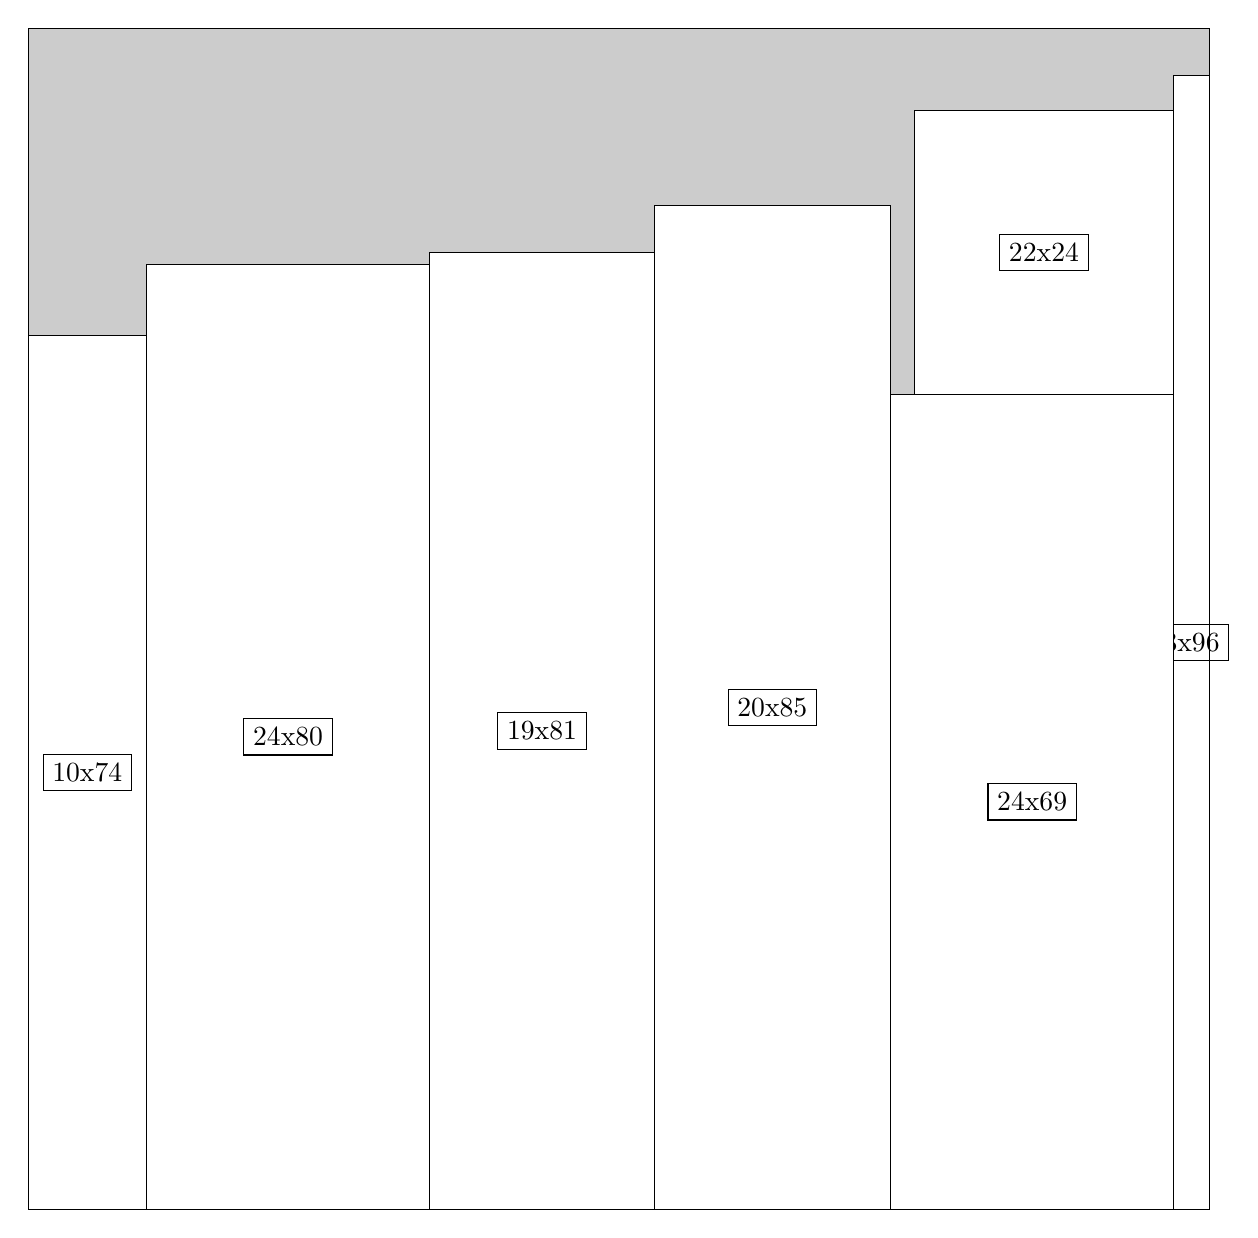
\begin{tikzpicture}[shorten >=1pt,scale=1.0,every node/.style={scale=1.0},->]
\tikzstyle{vertex}=[circle,fill=black!25,minimum size=14pt,inner sep=0pt]
\filldraw[fill=gray!40!white, draw=black] (0,0) rectangle (15.0,15.0);
\foreach \name/\x/\y/\w/\h in {3x96/14.549999999999999/0.0/0.44999999999999996/14.399999999999999,24x69/10.95/0.0/3.5999999999999996/10.35,22x24/11.25/10.35/3.3/3.5999999999999996,20x85/7.949999999999999/0.0/3.0/12.75,19x81/5.1/0.0/2.85/12.15,24x80/1.5/0.0/3.5999999999999996/12.0,10x74/0.0/0.0/1.5/11.1}
\filldraw[fill=white!40!white, draw=black] (\x,\y) rectangle node[draw] (\name) {\name} ++(\w,\h);
\end{tikzpicture}


w =3 , h =96 , x =97 , y =0 , v =288
\par
w =24 , h =69 , x =73 , y =0 , v =1656
\par
w =22 , h =24 , x =75 , y =69 , v =528
\par
w =20 , h =85 , x =53 , y =0 , v =1700
\par
w =19 , h =81 , x =34 , y =0 , v =1539
\par
w =24 , h =80 , x =10 , y =0 , v =1920
\par
w =10 , h =74 , x =0 , y =0 , v =740
\par
\newpage


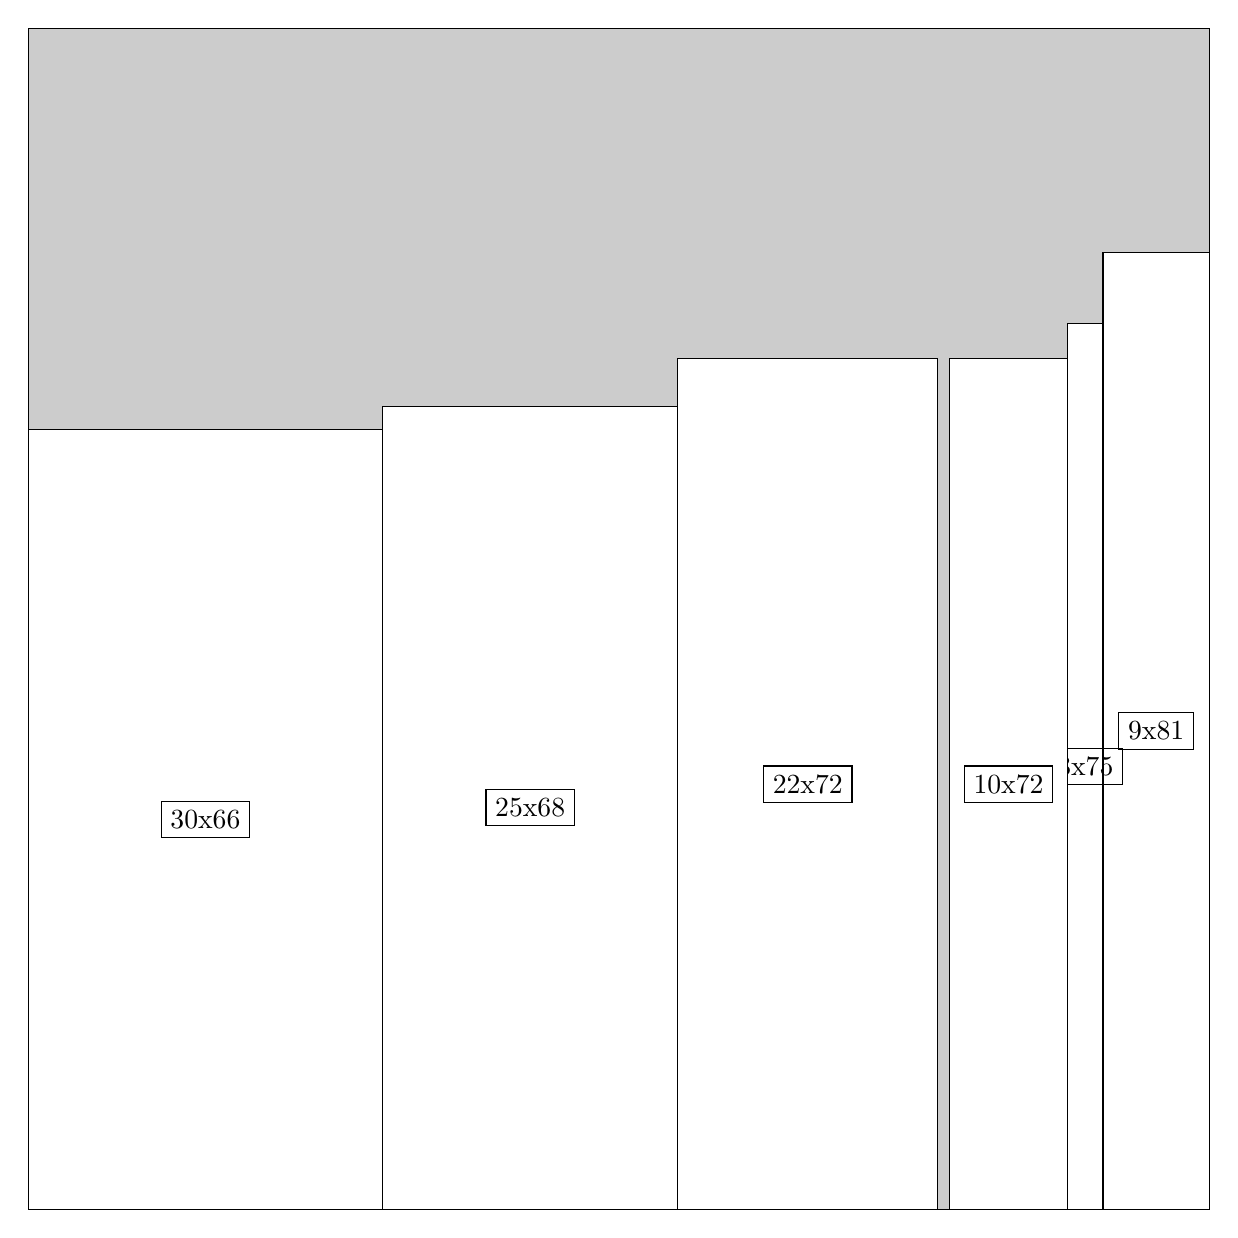
\begin{tikzpicture}[shorten >=1pt,scale=1.0,every node/.style={scale=1.0},->]
\tikzstyle{vertex}=[circle,fill=black!25,minimum size=14pt,inner sep=0pt]
\filldraw[fill=gray!40!white, draw=black] (0,0) rectangle (15.0,15.0);
\foreach \name/\x/\y/\w/\h in {9x81/13.65/0.0/1.3499999999999999/12.15,3x75/13.2/0.0/0.44999999999999996/11.25,10x72/11.7/0.0/1.5/10.799999999999999,22x72/8.25/0.0/3.3/10.799999999999999,25x68/4.5/0.0/3.75/10.2,30x66/0.0/0.0/4.5/9.9}
\filldraw[fill=white!40!white, draw=black] (\x,\y) rectangle node[draw] (\name) {\name} ++(\w,\h);
\end{tikzpicture}


w =9 , h =81 , x =91 , y =0 , v =729
\par
w =3 , h =75 , x =88 , y =0 , v =225
\par
w =10 , h =72 , x =78 , y =0 , v =720
\par
w =22 , h =72 , x =55 , y =0 , v =1584
\par
w =25 , h =68 , x =30 , y =0 , v =1700
\par
w =30 , h =66 , x =0 , y =0 , v =1980
\par
\newpage


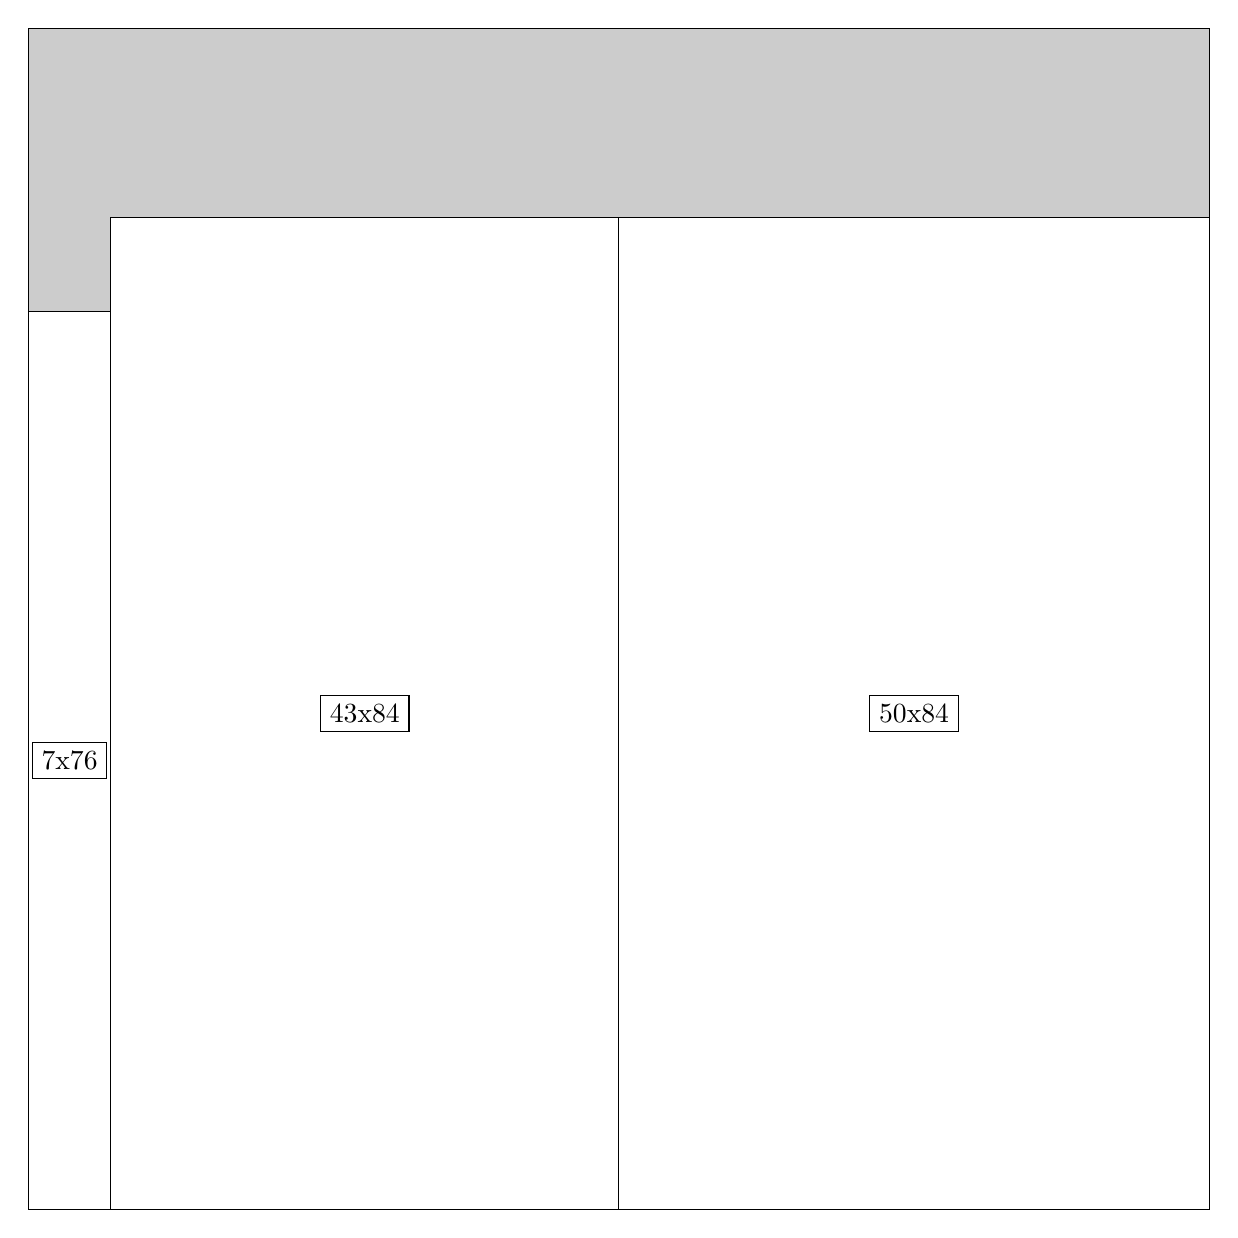
\begin{tikzpicture}[shorten >=1pt,scale=1.0,every node/.style={scale=1.0},->]
\tikzstyle{vertex}=[circle,fill=black!25,minimum size=14pt,inner sep=0pt]
\filldraw[fill=gray!40!white, draw=black] (0,0) rectangle (15.0,15.0);
\foreach \name/\x/\y/\w/\h in {50x84/7.5/0.0/7.5/12.6,43x84/1.05/0.0/6.45/12.6,7x76/0.0/0.0/1.05/11.4}
\filldraw[fill=white!40!white, draw=black] (\x,\y) rectangle node[draw] (\name) {\name} ++(\w,\h);
\end{tikzpicture}


w =50 , h =84 , x =50 , y =0 , v =4200
\par
w =43 , h =84 , x =7 , y =0 , v =3612
\par
w =7 , h =76 , x =0 , y =0 , v =532
\par
\newpage


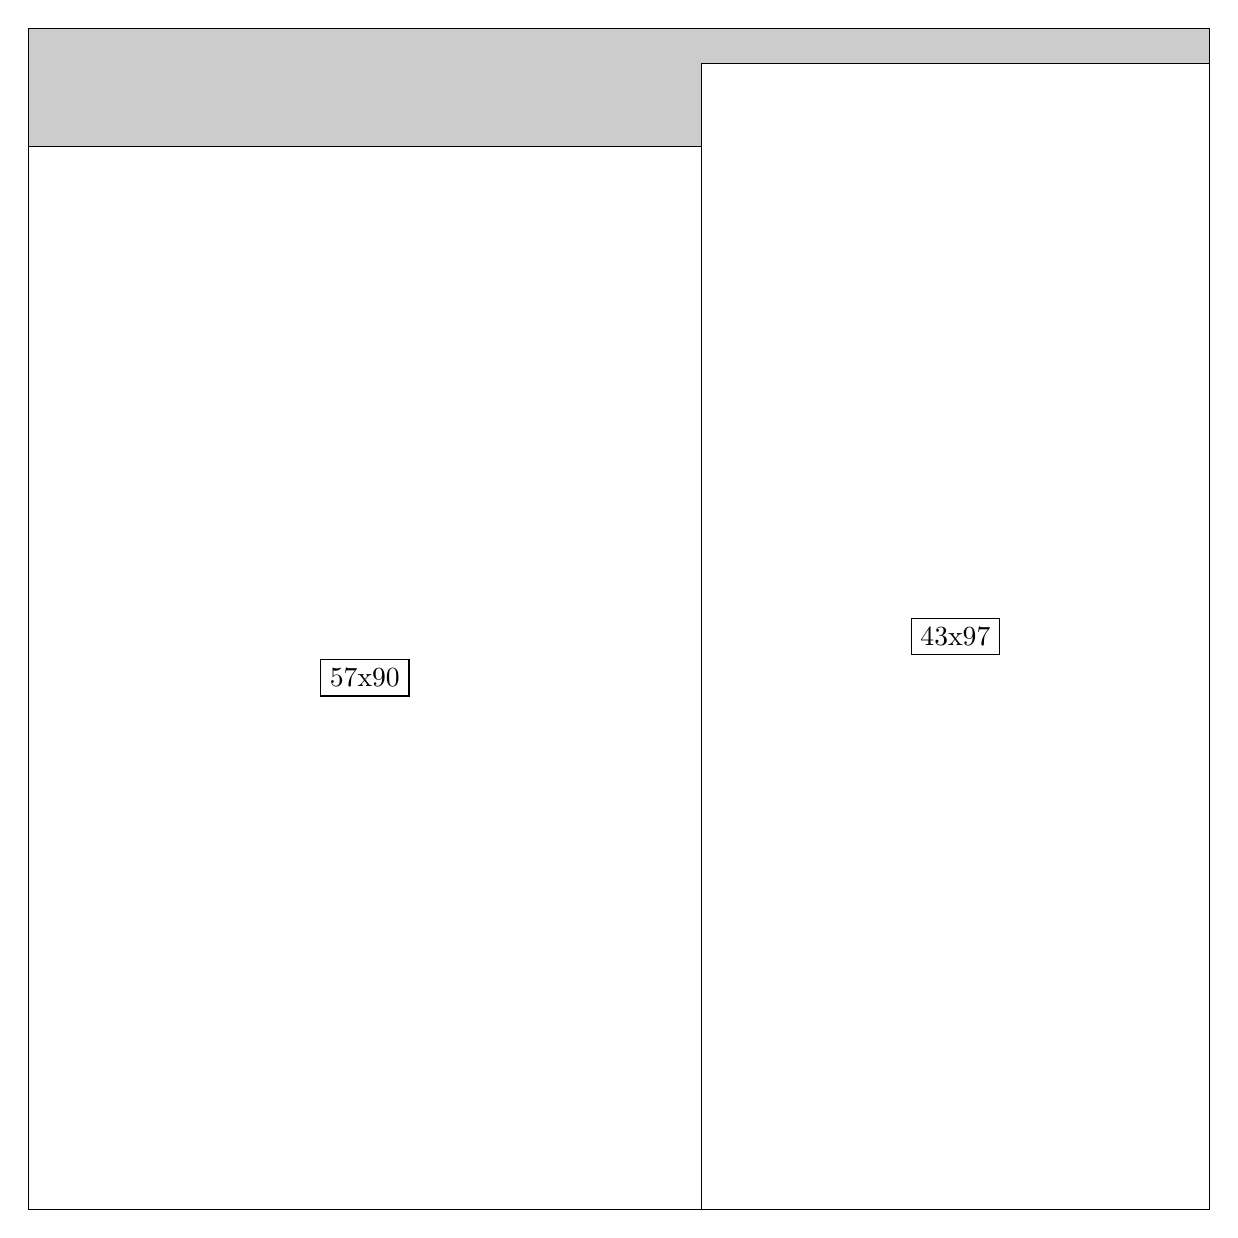
\begin{tikzpicture}[shorten >=1pt,scale=1.0,every node/.style={scale=1.0},->]
\tikzstyle{vertex}=[circle,fill=black!25,minimum size=14pt,inner sep=0pt]
\filldraw[fill=gray!40!white, draw=black] (0,0) rectangle (15.0,15.0);
\foreach \name/\x/\y/\w/\h in {43x97/8.549999999999999/0.0/6.45/14.549999999999999,57x90/0.0/0.0/8.549999999999999/13.5}
\filldraw[fill=white!40!white, draw=black] (\x,\y) rectangle node[draw] (\name) {\name} ++(\w,\h);
\end{tikzpicture}


w =43 , h =97 , x =57 , y =0 , v =4171
\par
w =57 , h =90 , x =0 , y =0 , v =5130
\par
\newpage


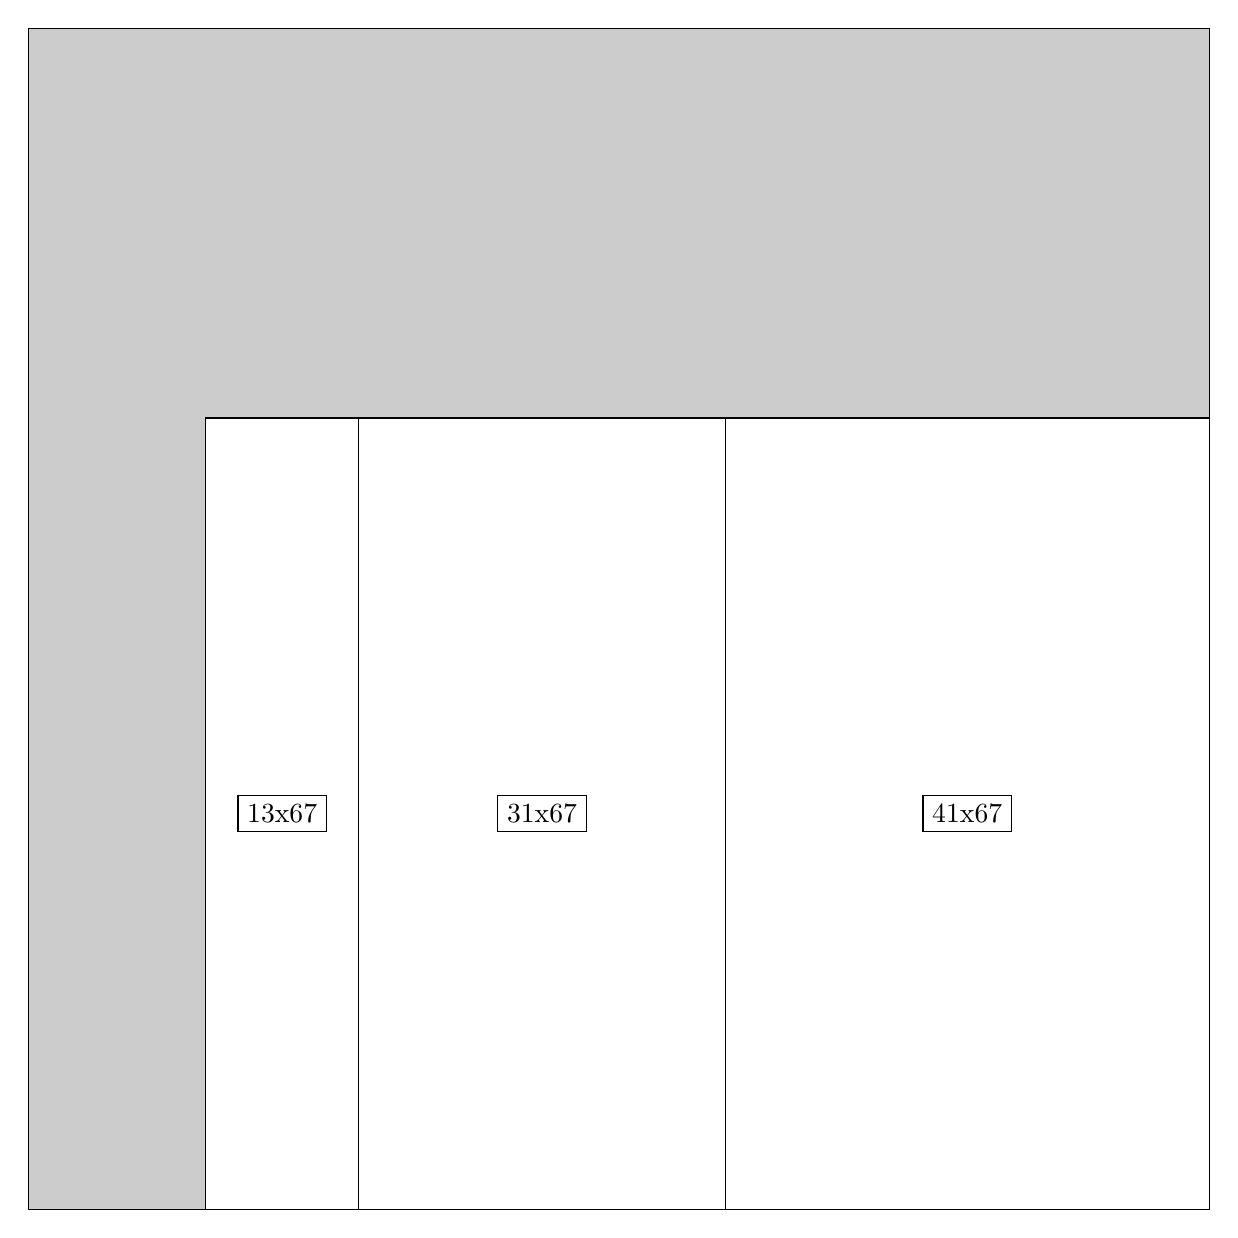
\begin{tikzpicture}[shorten >=1pt,scale=1.0,every node/.style={scale=1.0},->]
\tikzstyle{vertex}=[circle,fill=black!25,minimum size=14pt,inner sep=0pt]
\filldraw[fill=gray!40!white, draw=black] (0,0) rectangle (15.0,15.0);
\foreach \name/\x/\y/\w/\h in {41x67/8.85/0.0/6.1499999999999995/10.049999999999999,31x67/4.2/0.0/4.6499999999999995/10.049999999999999,13x67/2.25/0.0/1.95/10.049999999999999}
\filldraw[fill=white!40!white, draw=black] (\x,\y) rectangle node[draw] (\name) {\name} ++(\w,\h);
\end{tikzpicture}


w =41 , h =67 , x =59 , y =0 , v =2747
\par
w =31 , h =67 , x =28 , y =0 , v =2077
\par
w =13 , h =67 , x =15 , y =0 , v =871
\par
\newpage


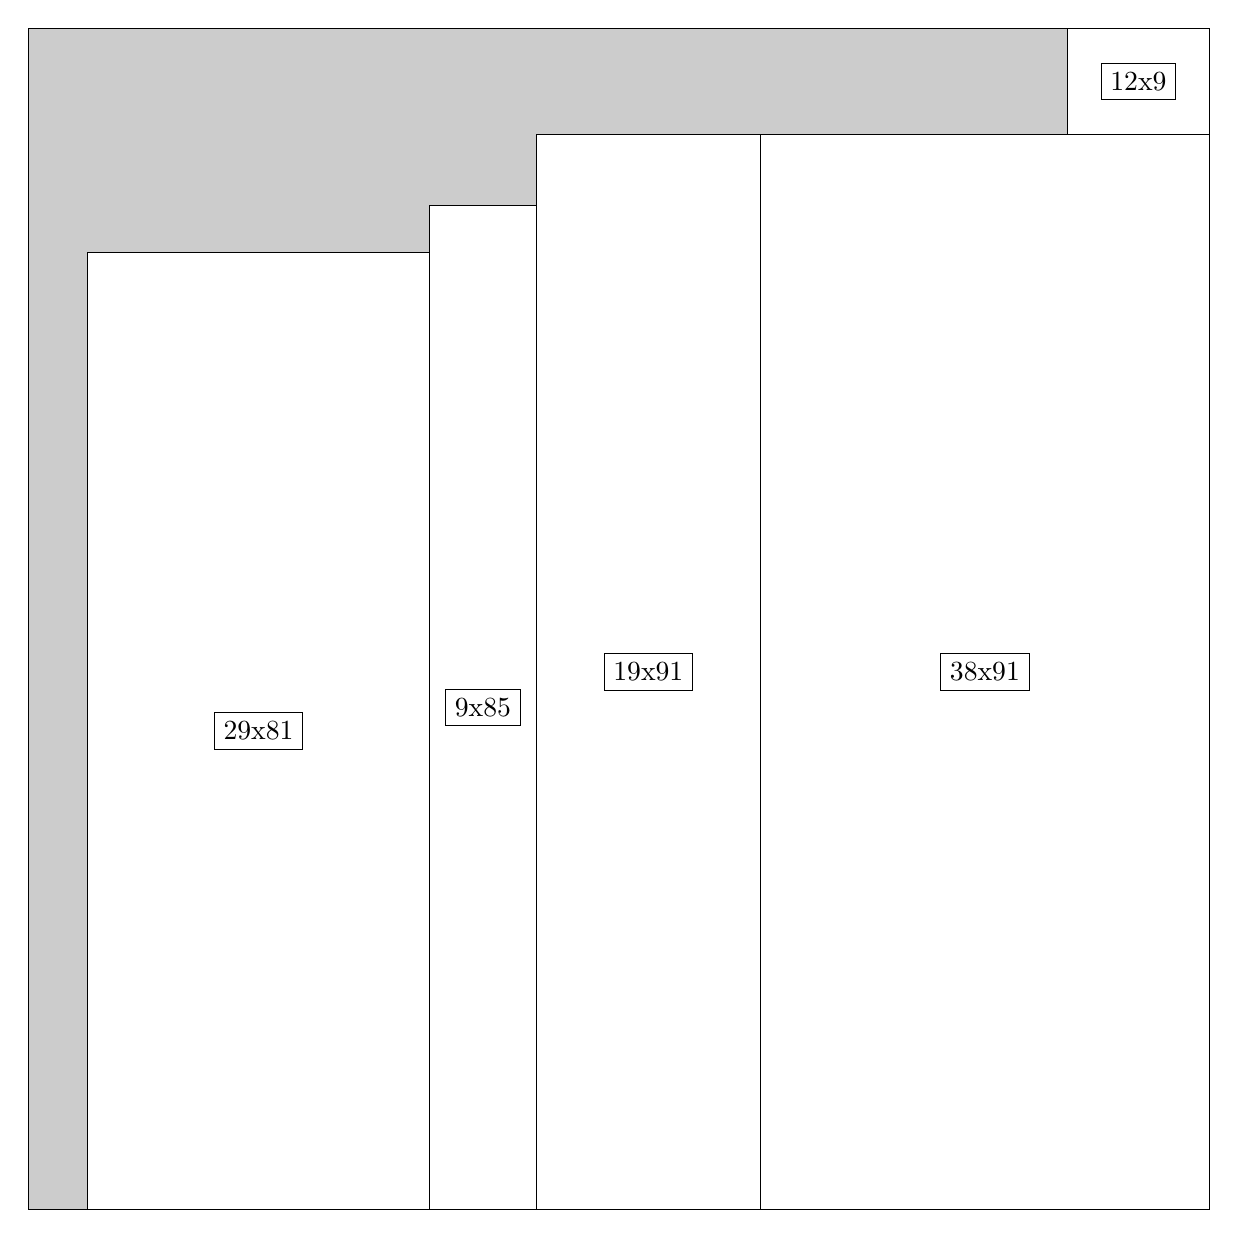
\begin{tikzpicture}[shorten >=1pt,scale=1.0,every node/.style={scale=1.0},->]
\tikzstyle{vertex}=[circle,fill=black!25,minimum size=14pt,inner sep=0pt]
\filldraw[fill=gray!40!white, draw=black] (0,0) rectangle (15.0,15.0);
\foreach \name/\x/\y/\w/\h in {38x91/9.299999999999999/0.0/5.7/13.65,12x9/13.2/13.65/1.7999999999999998/1.3499999999999999,19x91/6.45/0.0/2.85/13.65,9x85/5.1/0.0/1.3499999999999999/12.75,29x81/0.75/0.0/4.35/12.15}
\filldraw[fill=white!40!white, draw=black] (\x,\y) rectangle node[draw] (\name) {\name} ++(\w,\h);
\end{tikzpicture}


w =38 , h =91 , x =62 , y =0 , v =3458
\par
w =12 , h =9 , x =88 , y =91 , v =108
\par
w =19 , h =91 , x =43 , y =0 , v =1729
\par
w =9 , h =85 , x =34 , y =0 , v =765
\par
w =29 , h =81 , x =5 , y =0 , v =2349
\par
\newpage


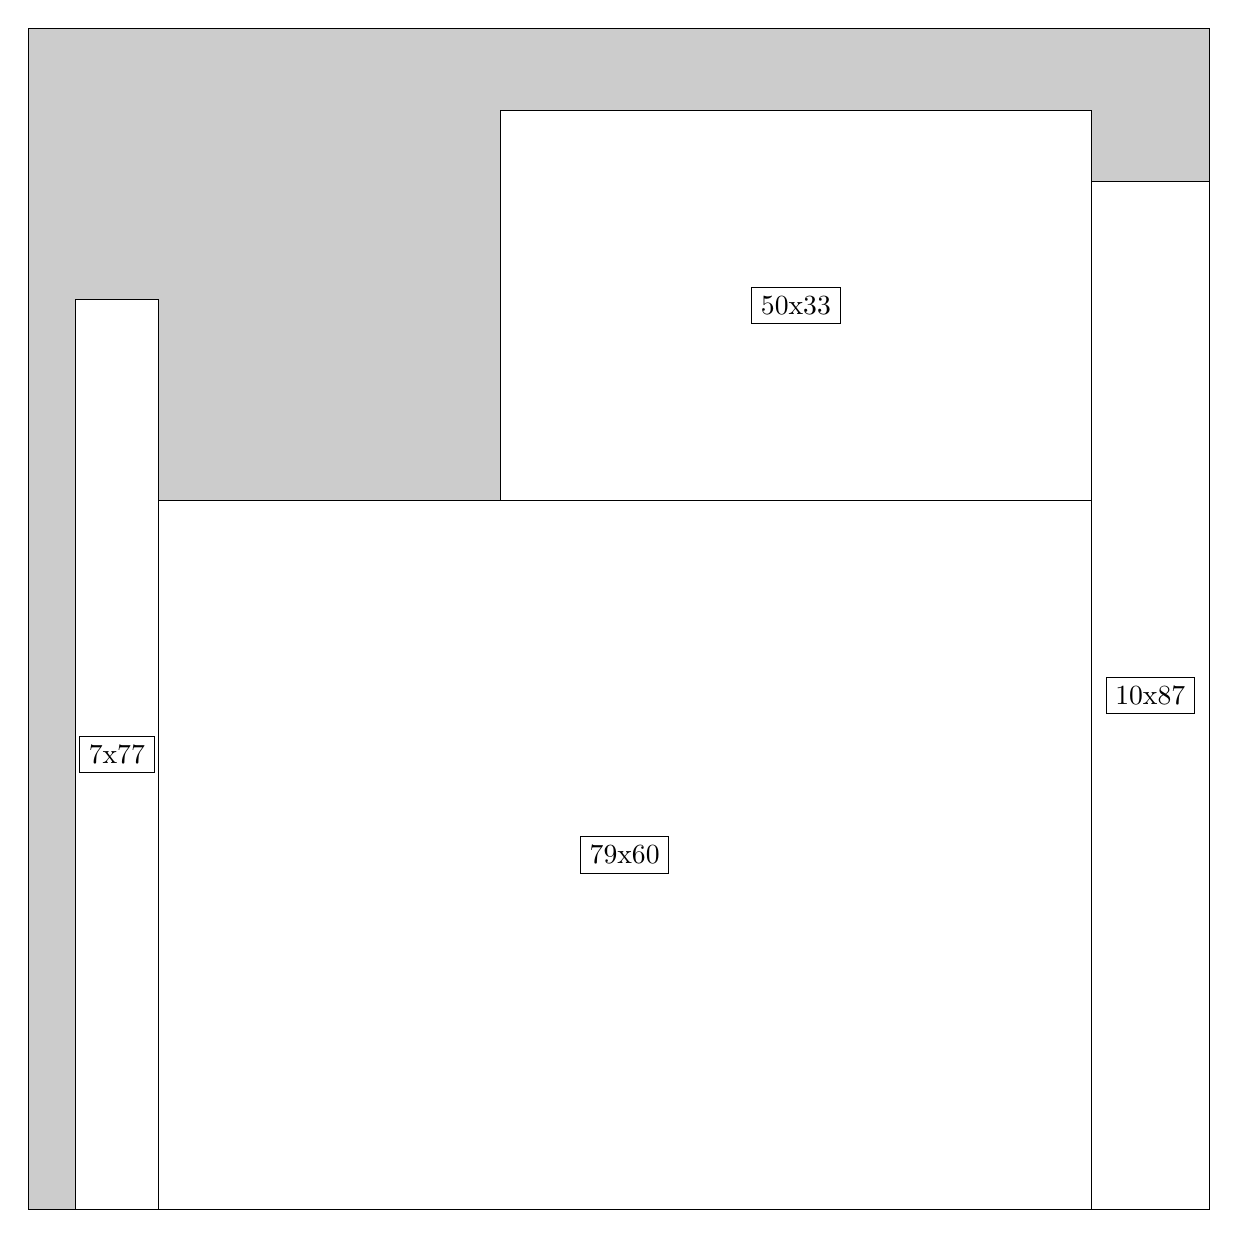
\begin{tikzpicture}[shorten >=1pt,scale=1.0,every node/.style={scale=1.0},->]
\tikzstyle{vertex}=[circle,fill=black!25,minimum size=14pt,inner sep=0pt]
\filldraw[fill=gray!40!white, draw=black] (0,0) rectangle (15.0,15.0);
\foreach \name/\x/\y/\w/\h in {10x87/13.5/0.0/1.5/13.049999999999999,79x60/1.65/0.0/11.85/9.0,50x33/6.0/9.0/7.5/4.95,7x77/0.6/0.0/1.05/11.549999999999999}
\filldraw[fill=white!40!white, draw=black] (\x,\y) rectangle node[draw] (\name) {\name} ++(\w,\h);
\end{tikzpicture}


w =10 , h =87 , x =90 , y =0 , v =870
\par
w =79 , h =60 , x =11 , y =0 , v =4740
\par
w =50 , h =33 , x =40 , y =60 , v =1650
\par
w =7 , h =77 , x =4 , y =0 , v =539
\par
\newpage


\end{document}